\documentclass[12pt,examcopy]{uathesis}
\usepackage{graphicx}
\usepackage{algorithm}
\usepackage{algpseudocode}
\usepackage{amssymb}
\usepackage{moreverb}
\usepackage{booktabs}
\usepackage{float}
\usepackage{babel}
\usepackage{amsmath}
\usepackage{fancyhdr}
\usepackage{booktabs}
\usepackage{multirow}
\usepackage{siunitx}
\usepackage{algorithm}
\usepackage[utf8]{inputenc}
\usepackage[noend]{algpseudocode}
\usepackage{algorithmicx}
\usepackage{amsthm}
\usepackage[hyphens,spaces,obeyspaces]{url}
\theoremstyle{definition}
\newtheorem{definition}{Definition}[section]

\usepackage{caption} 
\captionsetup[table]{skip=5pt}

\usepackage{hyperref}
\hypersetup{
    colorlinks,
    citecolor=blue,
    filecolor=blue,
    linkcolor=blue,
    urlcolor=blue
}

%newtheorem{algorithm}{Algorithm}[chapter]
\newtheorem{theorem}{Theorem}[section]
\newtheorem{corollary}{Corollary}[theorem]
\newtheorem{lemma}[theorem]{Lemma}

\usepackage{tikz}
\usetikzlibrary{shapes,arrows}
\usetikzlibrary{decorations.shapes}

% some settings to fill pages more densely
\renewcommand\floatpagefraction{.9}
\renewcommand\topfraction{.9}
\renewcommand\bottomfraction{.9}
\renewcommand\textfraction{.1}
\setcounter{totalnumber}{50}
\setcounter{topnumber}{50}
\setcounter{bottomnumber}{50}



\begin{document}
\title{Adaptive Self-Sufficient Itemset Miner for Transactional Data Streams}
\author{Francis Tang}
\department{Computer Science}
\supervisor{David T.J. Huang}{Yun Sing Koh}
\maketitle

\frontmatter
\begin{abstract}
\addcontentsline{toc}{chapter}{Abstract}
Most studies on pattern mining consider itemsets that have a high frequency of occurrence as useful, often determined by the support of the itemsets. However, current research has shown that we need to move beyond a pure ``support-confidence" framework for pattern mining. Recently, there is an interest on finding statistically significant patterns and one of the most popular type of patterns is self-sufficient itemsets. One limitation is that these works do not consider concept drifts and cannot be used in a data stream. Learning in the online environment requires us to develop efficient and effective mechanisms to address the online characteristics of non-static data and non-stationary data distributions. In our research we will concentrate on detecting self-sufficient itemsets from data streams. The usefulness of these itemsets are not solely determined by the frequency of either their subsets or their supersets. We present a comprehensive framework for mining self-sufficient itemsets from data streams along with a drift detector. This supports mining self-sufficient itemsets in an online environment and provides the ability to adapt to changes in the stream.
\end{abstract}

\begin{acknowledgements}
\addcontentsline{toc}{chapter}{Acknowledgements}
As my honours year comes to the end, first and foremost I would like to thank my extraordinary supervisors, David Huang and Yun Sing Koh for all of their wonderful care and patient guidance with me throughout this year. Even before I started studying this year, the way that you explained my project to me really inspired me to undertake my honours year in the pattern mining field. 

David, you taught me how to read tons of research papers, organise my research project and provided me constant help getting me familiar with new definitions which I got totally puzzled from the beginning and I am so grateful of this. To Yun Sing also, there are too many things to say thank you for this year but thank you for always reminding me and assisting me in writing my conference paper. You both really did provide me with all the background knowledge and technical support which made every experiment possible. Also, when it came time to write my paper and dissertation, both of you were unbelievably helpful in developing my critical scientific writing strategies and for staying up late to get it all finished. Without you, none of my work this year would have been achieved. All the feedback and support you provided me along the way allowed me to progress smoothly through this year even when I was completely lost. I am so glad to have had you as my supervisors.

I would also like to thank every other postgraduate student who I call my dear friends in the department for their assistance with all of the technical aspects of my experiments and for making me laugh when I was super stressed. Specifically, I would like to thank Jackie Excell and Edith Yi for all of their support during the year. Jackie taught me all the statistical skills I needed and Edith used her excellent programming skills to enlighten me hundreds of times when I was stuck.

Last but not the least, I would like to thank my best friends Iris and Huan. Thank you for all of the time you spent with me this year, the ‘comfort foods’ when I was sick, your support and for making me feel better when I was really low.

To mum at home, thanks so much for not only giving me financial support but also your unconditional love to support and guide me through this year. I hope I have made you proud.

\end{acknowledgements}

\listoffigures
\addcontentsline{toc}{chapter}{List of Figures}
 
\listoftables
\addcontentsline{toc}{chapter}{List of Tables}

\newpage

\renewcommand{\abstractname}{List of Publication}
\begin{abstract}

    \addcontentsline{toc}{chapter}{List of Publication}
    Parts of this dissertation has been accepted for publication:
    \begin{itemize}
    \item Feiyang Tang, David T.J. Huang, Yun Sing Koh and Philippe Fournier-Viger. Adaptive Self-Sufficient Itemset Miner for Transactional Data Streams. In \textit{The $16^t^h$ Pacific Rim International Conference on Artificial Intelligence (PRICAI)}, 2019 (Core Ranking B).
    \end{itemize}
\end{abstract}%




\setcounter{tocdepth}{2}
\tableofcontents

\mainmatter
\chapter{Introduction} \label{chapt:Introduction}
People recognise concepts, rules, restraints, and information as `knowledge'. Data is often treated as the basis of constructing knowledge. Traditionally, data mining and knowledge discovery was performed manually. As time passed, the amount of data in many systems grew to larger than terabyte size, and could no longer be maintained manually, which brought the idea of machine learning and data mining, also formed a part of artificial intelligence.

%Raw data can be structured, which means it resides in relational databases, like the information stored in a university's enrolment database. It can also be semi-structured, that does not conform with the formal structure of data models associated with relational databases or other forms of data tables, for instance, textual, graphical and image data. 

The process of knowledge discovery has been widely discussed since late $20^t^h$ century and focused on acquiring knowledge that is accurate and precise. The latter focus emphasises the execution efficiency of the algorithms. This may be achieved by adopting a more efficient data structure or having a faster processing mechanism.

\section{Big data and Data Mining}

Big data consists of large datasets that often exceed the collection, utilisation, management, and processing capabilities of humans within acceptable times. The size of big data often may vary. As in 2012, the size of a single dataset ranges from a few terabytes (TB) to tens of petabytes (PB) \cite{wiki:bigdata}.

Doug Laney \cite{bigdata}, an analyst at META Group (now Gartner) in 2001, articulated the challenges and opportunities for data growth have three directions: volume, variety, and velocity, collectively referred to as ``3V'' or ``3Vs'' \cite{bigdata}. Gartner and most of the companies in the big data industry today continue to use 3V to describe big data. Gartner revised the definition of big data in 2012 as: ``Big data is a large, high-speed and changeable information asset that requires new ways of processing to enable better decision making, insight and optimisation.'' In addition, there is the fourth V has been recently defined outside the 3V: veracity, to make an up-to-date definition: ``4V''. The ``4V'' definition is explained as following:

\begin{itemize}
    \item \textbf{Volume}. Organisations collect data from a variety of sources, including business transactions, social media and information from sensor or machine-to-machine data. In the past, storing it would have been a problem – but new technologies (such as Hadoop) have eased the burden.
    
    \item \textbf{Velocity}. Data streams in at an unprecedented speed and must be dealt with in a timely manner. RFID tags, sensors and smart metering are driving the need to deal with torrents of data in near-real time.
    
    \item \textbf{Variety}. Data comes in all types of formats – from structured, numeric data in traditional databases to unstructured text documents, email, video, audio, stock ticker data and financial transactions.
    
    \item \textbf{Veracity}. Big data veracity refers to the biases, noise and abnormalities, ambiguities, latency in data.
    
\end{itemize}

Big data must be statistically collected, compared, and parsed to a computer to produce objective results. The United States started to emphasise their research on big data in 2012. In the same year, President Obama invested 200 million dollars in the development of big data analytical projects, and emphasised that big data will be the future petroleum. 

As we all know, big data is not simply a fact of big data, but the most important is how to analyse big data. We can only get intelligent, in-depth and valuable information through data analysis. There are several methodologies that are common in big data analysis:

\begin{enumerate}

    \item \textbf{Visualisation}. As the target audience of big data analysis report may not be statistics or computer science professionals, it is very important to ensure that the information provided are relevantly direct and understandable. This brings visualisation in the first priority, because visualisation can intuitively present big data features and can be understand is as simple and straightforward as reading a picture.
    
    \item \textbf{Data mining algorithms}. The theoretical core of big data analysis is data mining algorithms. Various data mining algorithms based on different data types and formats can present the characteristics of the data more scientifically. The algorithms can usually achieve good efficiency which can significantly improve the cost of big data analysis.
    
    \item \textbf{Prediction}. One of the most important goals of big data analysis is to make predictions. After the characteristics are extracted from big data, data scientist can build a model based on these characteristics and predict the future trends. 
    
    \item \textbf{Big data management}. Big data analysis is inseparable from keeping the integrity and quality of input data. High-quality data and an effective data management will be beneficial in both academic research and commercial development, to ensure the authenticity and value of the results.
    
\end{enumerate}

Data mining, also as known as Knowledge Discover in Database (KDD), is the process of extracting information that is hidden from the prior art, but is potentially useful, from a large number of incomplete, noisy, fuzzy, and random practical data. This definition includes several layers of meaning: the data source must be real, large, and noisy; the knowledge that is of interest to users; the knowledge found is acceptable, understandable, and usable.

In the next section, we are going to look at data stream mining by defining data stream first then discuss some unique characteristic of data stream and how to make proper analysis on it.

\section{Data Stream Mining}

Data stream is ubiquitous in our lives. The telephone communication records, social media use, retail sales transactions and even the real-time stock exchange information are all data streams.

What is a data stream? We can understand that the data in these situations mentioned above have a common feature, that is, infinity. In addition to endless incoming data, think about the retail transactions and stock exchange records, they both have a very fast updating speed, which makes the timing critical for data stream analysis. The data first seen in the data stream could be expired after new data arrives. 

To understand and analyse the characteristics of the data stream, we naturally think, can we apply the traditional data mining method to data stream? As several mature data mining methods have developed during the last decades, data source is stored in flat files, relational databases, transactional databases, etc. These methods (such as OLAP) are built on top of data that has been saved statically and not updated frequently, for example, a data warehouse. Furthermore, some of our methods requires more than one access to the data. However, it is almost impossible to store data stream because of its infinite size and consistent updates. Aim to process a special type of data like data stream, it is better to scan the data once or a constant number of times but not the entire data stream to reduce the memory use. 

\subsection{Association Rule Mining}
For the successful existence of any business, discovering underlying patterns in data is considered essential. As a result, several pattern mining algorithms were developed to discover hidden data and make assumptions, which formed a part of artificial intelligence. These algorithms are able to find either the features which occur together or those are somehow correlated. 

What does the value of one feature tell us about the value of another feature? For example, people who buy nappies are likely to buy baby powder. Or we can rephrase the statement by saying: if (people buy nappies), then (they buy baby powder). Note the if, then rule. This does not necessarily mean that if people buy baby powder, they buy nappies. In General, we can say that if condition A tends to B it does not necessarily mean that B tends to A. The relationship between nappies and baby powder can be treated as an association rule, that is the interesting patterns we aim to mine from data streams.

Section~\ref{chapt:RelatedWorks} will have more discussion on the techniques which have been widely researched and used on data stream mining especially on association rule mining. To better mining significant patterns out from data stream, we will address out motivation in the next section.


\section{Motivation}

One of the most researched fields for data stream is mining significant patterns out of data stream. Current research in data stream pattern mining relies on using minimum or maximum support thresholds to derive the association rules~\cite{kingfisher}, which comes with many drawbacks such as not considering the statistical significance of patterns. Thus, these work may find many frequent patterns that are spurious - contains values that appear together by chance rather than having a strong correlation. To solve this drawback, Webb et al. \cite{ssi,topk} proposed and defined self-sufficient itemsets to produce more `interesting' rules. Those are itemsets having a frequency that cannot be explained solely by the frequency of their subsets or supersets. It has been shown that itemsets derived using minimum support that does not also satisfy the definition of self-sufficient itemsets are unlikely to produce interesting rules. Given the infinite growth of data streams, we require the association rule mining algorithms to be workable on a data stream. 


While a large number of papers discussed mining interesting association rules from data streams, the non-stationary distributions problem has not been as widely dealt with in the pattern mining research domain. Changes in the underlying distribution may lead to changes in the relevant pool of itemsets over time, which will reduce the correctness of interesting rules mined. This is known as the concept drift problem. In this section, we look at official retail data from Stats NZ~\cite{statsnz} which helps illustrate concept drift problems in data stream mining.

Figure \ref{fig:retail1} and \ref{fig:retail2} below are retail sales data in two different quarters: December 2017 to March 2018 and March 2018 to June 2018. It is very interesting to see that people buy significantly different goods in these two quarters. For instance, we look at sales of grocery, liquor and tobacco product from Quarter 1 2018 to Quarter 2 2018. The figures show us that sales went down in the first quarter of 2018 but went rapidly up during the second quarter. This kind of distribution changes bring the challenge of using a static model to mine patterns for a entire data stream. Obviously, changes need to be separately considered to ensure the accuracy of data stream pattern mining. 

\begin{figure}[H]
    \centering
    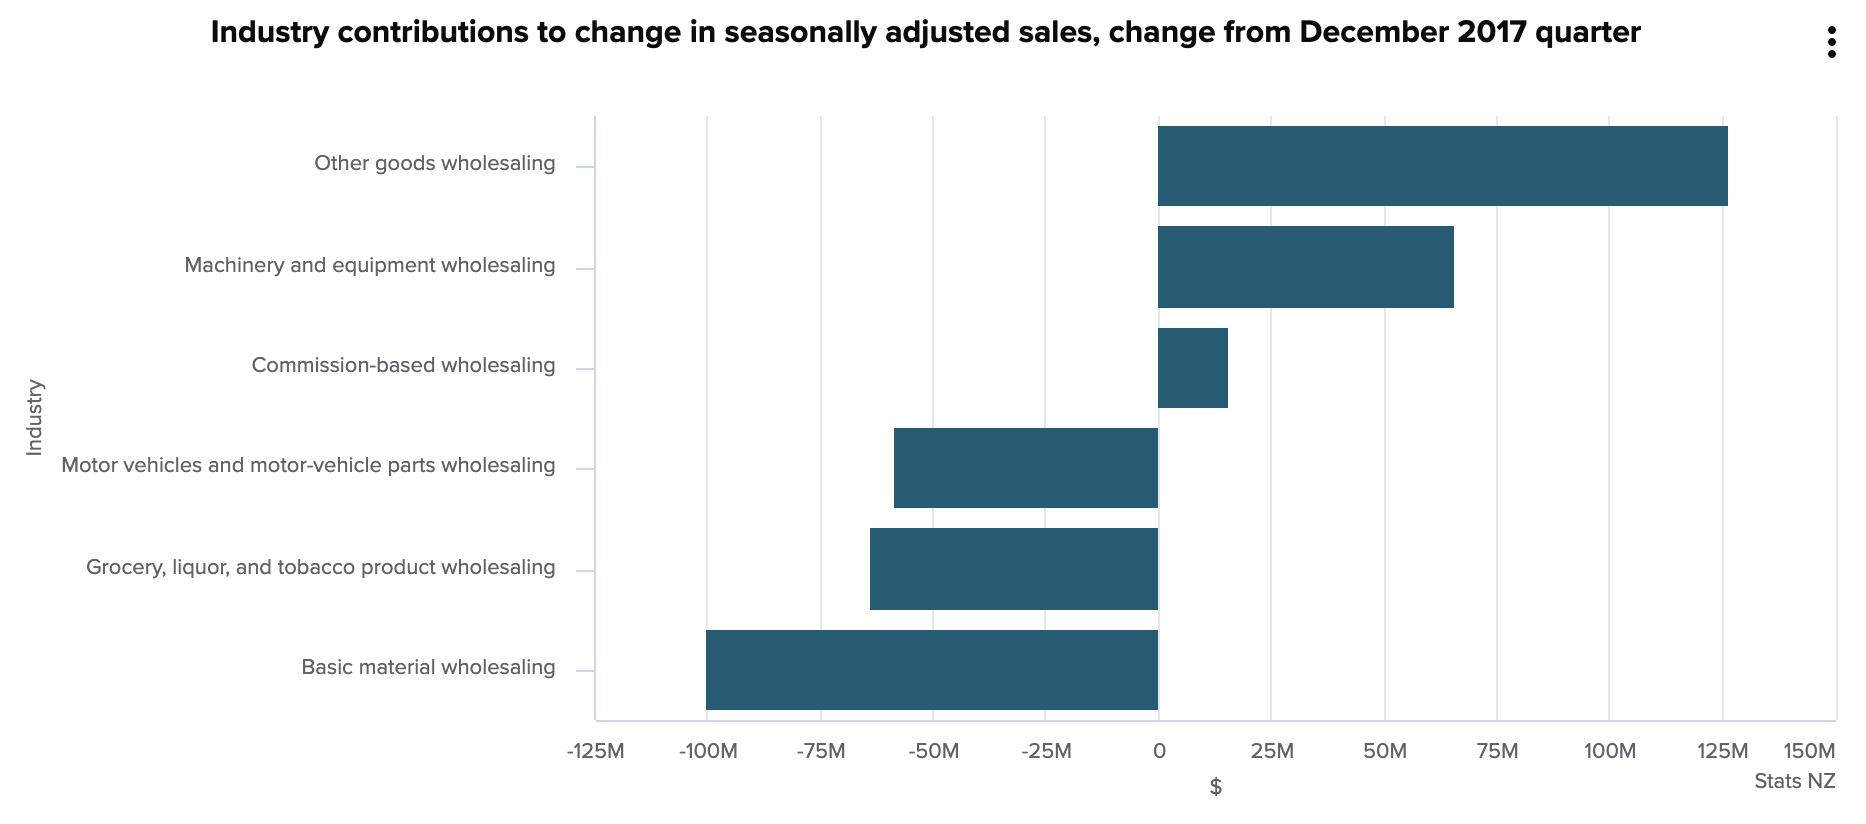
\includegraphics[width=\textwidth]{Introduction/1217to0318.png}
    \caption{NZ Retail data from 12-2017 to 03-2018 \cite{statsnz}}
    \label{fig:retail1}
\end{figure}

\begin{figure}[H]
    \centering
    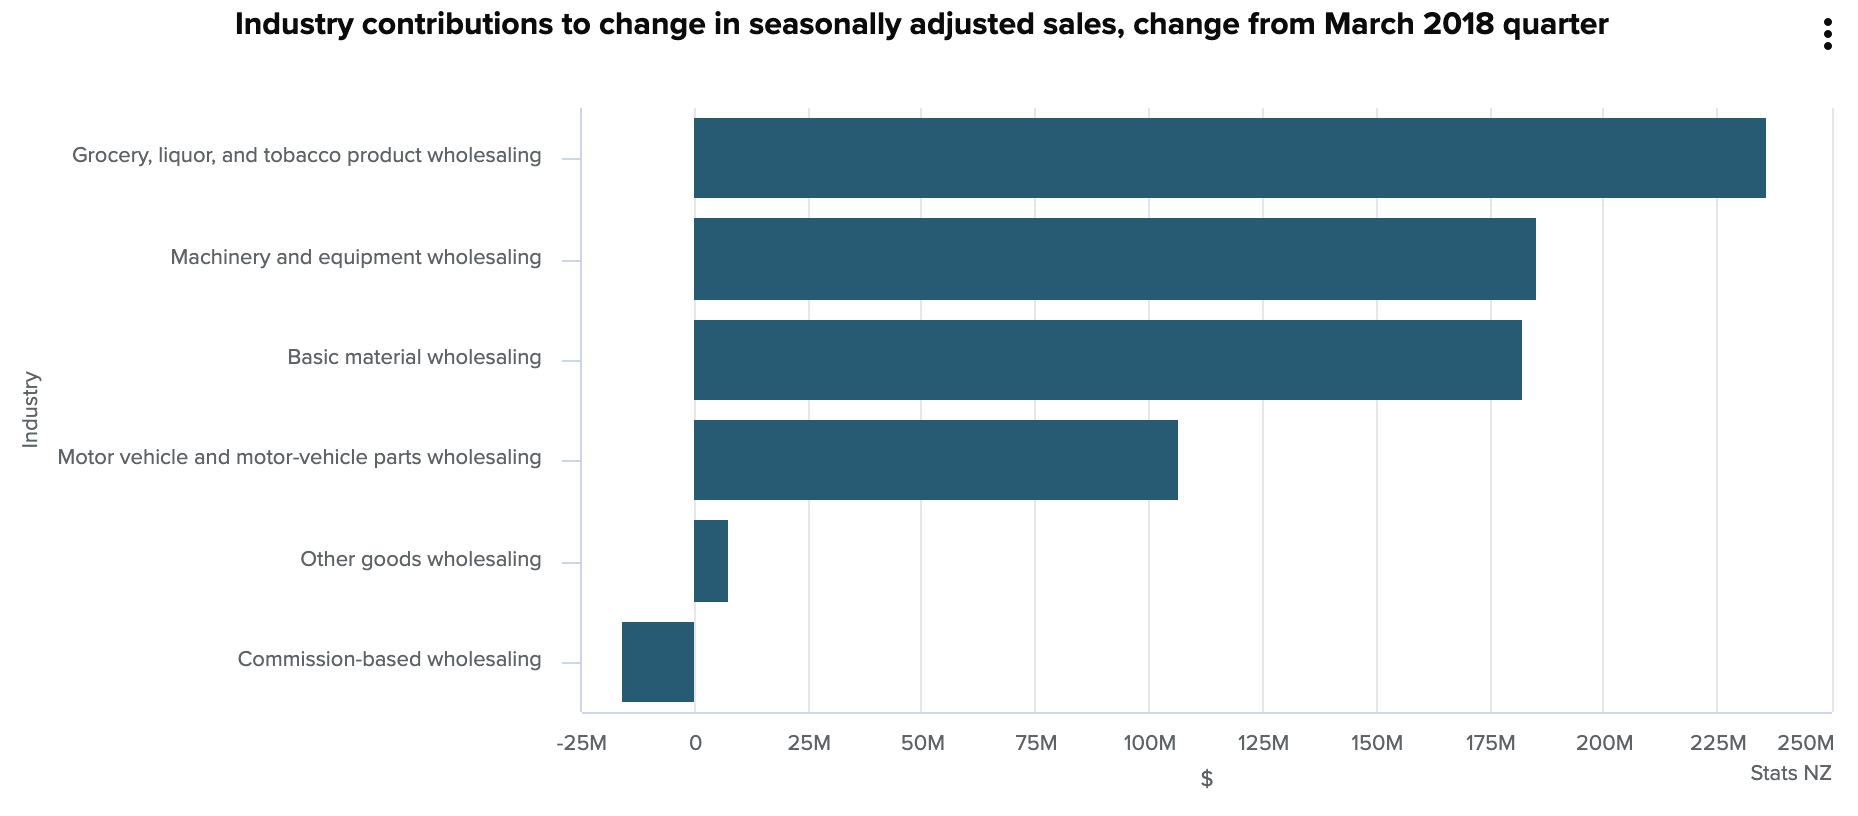
\includegraphics[width=\textwidth]{Introduction/0318to0618.png}
    \caption{NZ Retail data from 03-2018 to 06-2018 \cite{statsnz}}
    \label{fig:retail2}
\end{figure}



%Small work around example of regional drift 

Currently when a change is detected by the concept drift detector, the entire existing set of rules previously found are discarded and we re-mine the rules from the new data in the data stream. This is an inefficient method since there is a possibility that only a small portion of the rules have changed and discarding and re-mining entire sets to discover small changes is not ideal. There is also the problem of setting a proper interval value to discard and re-mine. If we discard and re-mine too frequently, the running cost will be high. One the other hand, if we discard and re-mine too infrequently, we risk not picking up the correct rules within the time-frame. For example, using supermarket basket analysis data, consider the situation where the supplier for Cheerios had suddenly stopped supplying Cheerios to the supermarket. As a consequence, future transactions will not contain Cheerios and this leads to a concept drift. If we discarded and re-mined at this time, the patterns containing Cheerios will be lost. If Cheerios immediately starts to restock after we re-mined, we are not able to pick up the patterns related to Cheerios again. Therefore, in this case, the disappearance of Cheerios could be identified as a regional drift. Mining regional drifts allow us to better adapt to the intricate changes in the patterns over time. 

\section{Research Questions and Objectives}
In this dissertation we study adaptive association rule mining in data streams. Adaptive association rule mining refers to updating learning models to react to the presence of changes. The prior sections list the background and motivations, the specific research questions that we look at are:

\subsection{Research Questions}
\begin{enumerate}
\item Why pure ``support-confidence'' framework is not sufficient to solve some real-world association rule mining problems?

\item Can we propose a working approach that facilitates the discovery of self-sufficient itemset accurately and efficiently in data streams.

\item Can we define and introduce the problem of detecting concept drift in self-sufficient itemset mining in data streams?

\item Can we develop a self-sufficient itemset mining technique that also detects and adapts to different kinds of concept drifts accurately and efficiently in data streams?
\end{enumerate}

\subsection{Objectives}
This dissertation focuses on developing algorithms that overcome the drawbacks of the ``support-confidence'' mining technique and adapt to different kinds of concept drifts to effectively acquire and learn knowledge from data streams. Our objectives are:

\begin{enumerate}
\item To address drawbacks of the pure ``support-confidence'' framework and compare it with improved techniques such as Self-Sufficient itemset.

\item To establish adaptive self-sufficient itemset mining using not only the pure support and confidence of items but also their associations with each other.

\item To develop a novel technique that detects and adapts to abrupt, gradual and regional concept drifts that occurs in data stream.

\item To develop an algorithm that solves the problem of mining self-sufficient itemset in an online mode along with concept drift adaption.
\end{enumerate}

\section{Contributions}

The main contributions made by this dissertation are:


\begin{enumerate}
\item I review work from several disciplines which may be of relevance to the present sub-ject of inquiry, and provide commentary on how the findings from these disciplines may be useful (Section~\ref{chapt:RelatedWorks}).

\item I provide a framework for mining self-sufficient itemset mining using not only the pure support and confidence of items but also their associations with each other. With this framework as a reference template, future work in this domain should be able to proceed more adaptive and accurate. (Section~\ref{chapt:ASSIM}).

\item By applying this framework to transactional data streams, I am able to detects and adapts to abrupt, gradual and regional concept drifts that occurs during the self-sufficient itemset mining process and adapt to those drifts. This allows future self-sufficient itemset mining achieve more accurate and stable results. (Section~\ref{chapt:ASSIM})

\end{enumerate}


\section{Structure of Dissertation}

This dissertation is structured into the following chapters:

\begin{itemize}
    
    \item \textit{Section~\ref{chapt:Introduction} Introduction}\newline
    We provide the reader with the relevant background to understand this dissertation.

    \item \textit{Section~\ref{chapt:RelatedWorks} Related Works}\newline
    We introduce relevant research in association rule mining, self-sufficient itemset, and concept drift mining. In particular, we detail seminal research and review the overall state of the current research. We also review the difference in the works pertaining to the traditional ``support-confidence'' technique versus the self-sufficient itemset discovery framework.
    
    \item \textit{Section~\ref{chapt:ASSIM} Self-sufficient Itemset Stream Mining}\newline
    We propose our Adaptive self-sufficient Itemset Miner (ASSIM) framework, discuss how its components interacts with each other, and explain how ASSIM improves the mining process of self-sufficient itemsets.
    
    \item \textit{Section~\ref{chapt:Experiments} Experiments}\newline
    We perform several experiments on evaluating the key components of ASSIM by comparing their computational costs, precision \& recall, and other important measures.
    
    \item \textit{Section~\ref{chapt:Conclusion} Conclusion}\newline
    We conclude the work, point out future directions and add some final reflections and remarks.
\end{itemize}


\chapter{Related Works} \label{chapt:RelatedWorks}

Association discovery \cite{arm1} is one of the most researched topics in data mining. However, the fielded applications appear to be relatively few, especially for applying association rule mining techniques to data streams, which becomes more common in real-world scenarios.

It has been suggested that this is due to the susceptibility of conventional association discovery techniques to finding large numbers of associations that are unlikely to be interesting to the user \cite{topk}. In this chapter I will survey and summarise the literature of association rule mining and how to detect and adapt to the concept drifts.

The structure of this chapter is as follows. Section \ref{sec:2.1} discusses basic knowledge of data streams. Section \ref{sec:2.2} discusses the preliminaries on association rule mining and some mainstream association rule mining techniques. Section \ref{sec:2.3} discusses basics of concept drift and several popular drift detectors. Section \ref{sec:2.4} explains the definition of self-sufficient itemset and why we adopted it in our proposed framework. Section \ref{sec:2.5} summarises this section.


\section{Data Stream Basics}\label{sec:2.1}
In this section, several basic definitions of data stream will be discussed first, followed by discussing the current general processing approaches.

A data stream is a sequence of data instances arriving continuously. It is considered to be dynamic and unbounded in size with data generated at a very fast pace. Generally, a dynamic data stream cannot be processed in the same way as a static database. Dynamic data streams requires one-pass techniques using either batch processing or online processing of data.

In this dissertation, our concentration is transactional data stream which consists infinite number of transactions.

%\theoremstyle{definition}
%\begin{definition}{Data Stream}
\begin{definition}[\textbf{\textit{Transactional Data Stream}}]
\label{datastream}
A data stream $\mathcal{D}$ with $n$ elements is defined as $\mathcal{D} = \{T_1, T_2, ..., T_n\}$, where by $T_i$ represents a transaction at time $i$. Each transaction contains a set of items $T = \{x_1, x_2, \ldots x_m\}$, where by $x_j$ represents an item. 
\end{definition}

Next, we will review the the mainstream processing approaches of data stream.

\subsection{Processing Approaches}
Due to the constraints of data streams: one-time access, continuous processing, limited memory, and fast response, data stream processing needs to be very efficient and computationally affordable. There are a number of different streaming methods proposed for data streams but there are two approaches that are predominantly considered: batch processing approach and sliding-window approach. Read et al. \cite{ds} provides a comparison of processing approaches in data streams.

\subsubsection{Batch processing approach}
Batch processing divides data stream into batches, different batches will be fed into mining techniques to solve tasks. The batch generation criteria can be time on how long data will be collected before dispatching processing on it or a fixed interval on data stream. 

\begin{figure}[H]
    \centering
    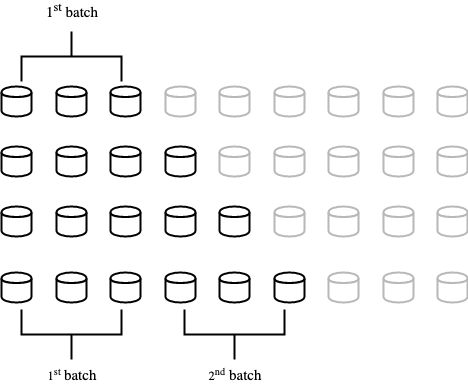
\includegraphics[width=0.6\textwidth]{RelatedWorks/batch.png}
    \caption{An example of batch processing approach}
    \label{fig:abrupt}
\end{figure}

\subsubsection{Sliding-window approach}
In the sliding window approach, data is processed after
the arrival of every single data instance. A sliding window generally has a fixed size and data is kept in the window based on the first in first out (FIFO) rule. The window moves when new data instance arrives, it slides to store the new data by dropping the oldest instance in the window, which keeps data in the window updated at any time point.

\begin{figure}[H]
    \centering
    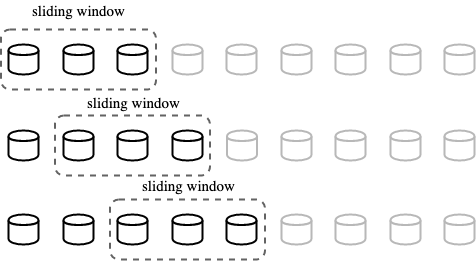
\includegraphics[width=0.6\textwidth]{RelatedWorks/window.png}
    \caption{An example of sliding-window approach}
    \label{fig:abrupt}
\end{figure}

\section{Association Rules} \label{sec:2.2}
To discover interesting patterns and relationships in data streams, association rules mining plays a key role in mining data streams. Firstly, the definition of frequent itemsets is introduced to help understand and create association rules.

\begin{definition}[\textbf{\textit{Frequent Itemset}}]
\label{freqitemset}
Frequent itemset, as it appears to mean, is itemset which appears frequently in a data stream. To determine if an itemset is frequent or not, the definition of support value is introduced: the support of an itemset $X$ with respect to data stream $\mathcal{D}$ with $n$ transactions is defined as the proportion of transactions $T$ in the dataset which contains the itemset $X$.
\end{definition}

\[ support(X)=\frac{|T \in \mathcal{D}, X \subseteq T|}{|n|} \]

Usually, a preset minimum support threshold is used to determine if an itemset is frequent or not. Once the support of an itemset surpass the minimum support threshold, it can be determined as a frequent itemset.

Here we use a sample database in Table \ref{tb:tidlist}, it consists five transactions with seven distinct items, and the minimum support threshold is set to 2.

\begin{table}[h!]
\caption{Set of Five Transactions}
\label{tb:tidlist}
\centering
 \begin{tabular}{p{6cm}} 
 \hline\hline
 \multicolumn{1}{c}{Transactions (tid: items)}\\
 \hline
 1: a, b, c, d, e \\ 
 %\hline
 2: a, b, c, d, f, h \\
 %\hline
 3: a, f, g \\
 %\hline
 4: b, e, f, g \\
 %\hline
 5: a, b, c, d, e, h \\
 \hline
\end{tabular}
\end{table}

\begin{definition}[\textbf{\textit{Association Rules}}]
\label{ar}
Association rules are if-then statements that help to show the probability of relationships between data items within data streams. They are calculated from itemsets, which are made up of two or more items, using the measure of \textit{support}, \textit{confidence} and \textit{lift}.
\end{definition}

To mine association rules, both LHS and RHS of a rule shall come from the frequent itemsets. Here another indicator \textit{confidence} level is introduced to indicate how often the rule has been found to be true.

The confidence value of a rule, $X \Rightarrow Y$, with respect to a set of transactions $T$, is the proportion of the transactions that contains $X$ which also contains $Y$.

\[confidence(X \Rightarrow Y) = \frac{support(X \cup Y)}{support(X)}\]

Similar to frequent itemsets, when the confidence of a rule surpasses the preset minimum confidence threshold, this rule might be labelled interesting.

\subsection{Join-based Association Rule Mining Algorithms}

The most basic join-based algorithm for association rule mining is Apriori algorithm \cite{apriori}. 

\begin{definition}[\textbf{\textit{Apriori}}]
\label{Apriori}
The key concept of Apriori algorithm is the anti-monotonicity of support value, it assumes that: all subsets of a frequent itemset must be all frequent.
\end{definition}

Apriori uses a breadth-first search strategy to count the support of itemsets and uses a candidate generation function which exploits the downward closure property of support. A simple example of Apriori algorithm is shown below in Figure \ref{fig:apriori} using data from Table \ref{tb:tidlist}.

\begin{figure}[H]
    \centering
    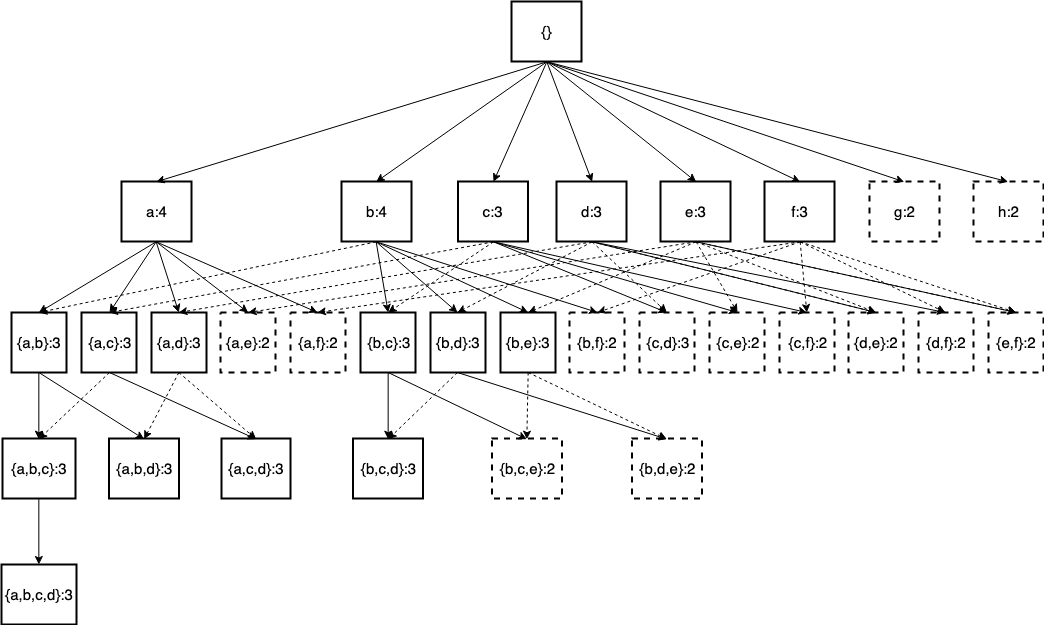
\includegraphics[width=1.0\textwidth]{RelatedWorks/apriori.png}
    \caption{An example of Apriori algorithm \cite{apriorifig}}
    \label{fig:apriori}
\end{figure}

Because of its very expensive computational cost of scanning the whole data and support counting, there are numerous optimisations proposed during the last two decades. Together with the proposal of the Apriori algorithm, Agrawal et al \cite{apriori} proposed AprioriTid and AprioriHybride as two practical optimisations. AprioriTid \cite{apriori} replaces every transaction in the database by the set of candidate itemsets that occur in that transaction, which significantly reduces the time consumed counting support values. AprioriHybrid combines Apriori and AprioriTid into a single hybrid which achieves a more flexible solution for association rule mining \cite{apriori}.

Rather than AprioriTid and AprioriHybrid, there are also other techniques proposed to optimise original Apriori algorithm, such as the work done in \cite{apriori2} and \cite{apriori3}.

To speed up the Apriori method, DHP algorithm, also known as Direct Hashing and Pruning method was proposed in 1995 \cite{DHP}.

\begin{definition}[\textbf{\textit{Direct Hashing and Pruning}}]
\label{DHP}
 There are two optimisations used in DHP \cite{DHP}. First, the candidate itemsets are going to be pruned when each new iteration happens. Second, not every whole transaction will be fed, there will be a trimming process of transactions to speed up the algorithm.
\end{definition}

To avoid meaningless itemsets when the next new candidate itemsets need to generated, DHP uses hash functions to remove them in advance. While Apriori requires to scan the entire database, which potentially massively increases the computational cost, DHP reduced the candidate itemset size. It has been proved that DHP performs significantly faster than the original Apriori algorithm.

Figure \ref{fig:dhp} below gives a simple example of how DHP works. In this case, we will not use the transactional data in Table \ref{tb:tidlist} which is going to need a very long hash table. Here we use a smaller database and perform DHP based on that. 

\begin{figure}[H]
    \centering
    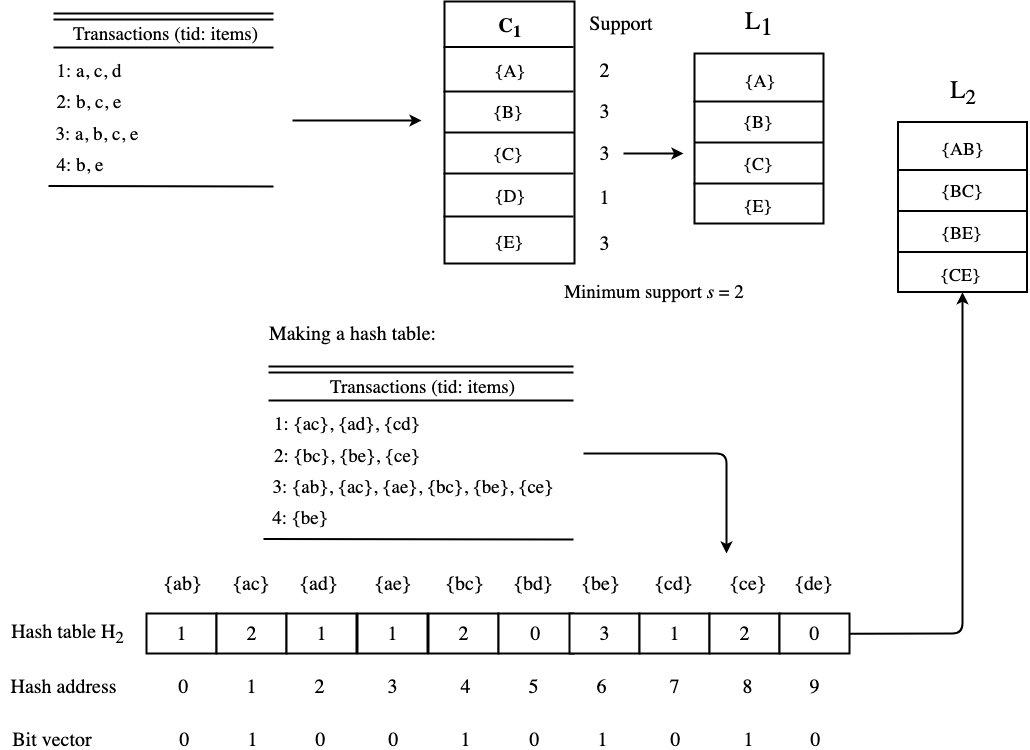
\includegraphics[width=1.0\textwidth]{RelatedWorks/DHP.png}
    \caption{An example of DHP algorithm \cite{DHP}}
    \label{fig:dhp}
\end{figure}

To reduce the computational cost of support counting in association rule mining is to find support of multiple frequent itemsets at one time. In 2004, Uno et al \cite{LCM} proposed LCM algorithm to use hyper-cube decomposition to achieve this goal. 

\begin{definition}[\textbf{\textit{LCM Algorithm}}]
\label{LCM}
The multiple itemsets obtained at the same one time, comprise a hypercube in the itemset lattice. For a frequent itemset $S$, let $H(S)$ be the set of items $a$ satisfying $a > tail(S)$ and transactions $T(S)=T(S\cup \{a\})$. Then, for any $P\subseteq H(S)$, $T(S\cup P)=T(S)$ holds, and $S\cup P$ is frequent. LCMfreq \cite{LCM} uses this property. For two itemsets $S$ and $S\cup P$, we say that $S'$ is between $S$ and $S\cup P$ if $S \subseteq S' \subseteq S \cup P$. In the iteration with respect to $S$, we output all $S'$ between $S$ and $S \cup H(S)$ \cite{LCM}.
\end{definition}

LCM saves about $2^{|H(S)|}$ times of the frequency counting \cite{LCM}.

\subsection{Tree-based Association Rule Mining Algorithms}

Another mainstream association mining technique is tree-based. They are based on set-enumeration concepts, which uses a subgraph of the lattice of itemsets to explore the candidate itemsets. Therefore, they will be used interchangeably, thus, the problem of generating frequent itemset will be constructing a enumeration tree.

\begin{definition}[\textbf{\textit{AIS Algorithm}}]
\label{AIS}
AIS algorithm was proposed by Agrawal et al \cite{arm2} in 1994, is basically a lexicographic tree algorithm. AIS constructs level-wise trees, itemsets are counting based on the transactional database with corresponding levels. AIS is a na\"ive mechanism, it searches the entire space without optimisation. 
\end{definition}

Many researchers proved that using vertical database layout could achieve significant performance improvements comparing to traditional intersection based counting techniques. Basically, for each transaction identifiers, one can have a list of items that are contained in it. And this is often referred as \textit{tidlist}. One of the earliest invention was Eclat proposed by Zaki \cite{eclat}. Here we will still use sample database in Table \ref{tb:tidlist} to illustrate the algorithms mentioned next, and the vertical representation of Table \ref{tb:tidlist} is shown in Table \ref{tb:tidlistvert} below. In this case, for instance, itemset $\{a,b\}$ can be computed as the length of the intersection of the \textit{tidlists} of $a$ and $b$.

\begin{table}[h!]
\caption{Vertical Presentation}
\label{tb:tidlistvert}
\centering
 \begin{tabular}{p{4cm}} 
 \hline\hline
 \multicolumn{1}{c}{Frequent Items (Item: \textit{tidlists})}\\
 \hline
 a: 1, 2, 3, 5 \\ 
 %\hline
 b: 1, 2, 4, 5 \\
 %\hline
 c: 1, 2, 5 \\
 %\hline
 d: 1, 2, 5 \\
 %\hline
 e: 1, 4, 5 \\
 f: 2, 3, 4\\
 g: 3, 4\\
 h: 2, 5\\
 \hline
\end{tabular}
\end{table}

\begin{definition}[\textbf{\textit{Eclat}}]
\label{eclat}
Eclat \cite{eclat} uses intersection based approach to calculate itemset support values in a vertical database. The partitioning approach is similar to Apriori algorithm \cite{apriori} but Eclat essentially generates candidate itemsets using only the join step from Apriori. 
\end{definition}

First, Eclat gets \textit{tidlist} for each item using DB scan. In this case, we use an item $a$ as an example. \textit{tidlist} of $a$ is exactly the list of transactions containing $a$. Next, Eclat intersects \textit{tidlist} of $a$ with \textit{tidlists} of all other items, resulting in \textit{tidlists} of $\{a,b\}, \{a,c\}, \{a,d\}$, which is called $a$-conditional database (removed $a$). Eclat repeats from 1 on $a$-conditional database and then repeats for all other items.

Figure \ref{fig:eclat} \cite{survey2014} illustrates the itemset generation tree with support computation by \textit{tidlist} intersection for transactions in Table \ref{tb:tidlist}.

\begin{figure}[H]
    \centering
    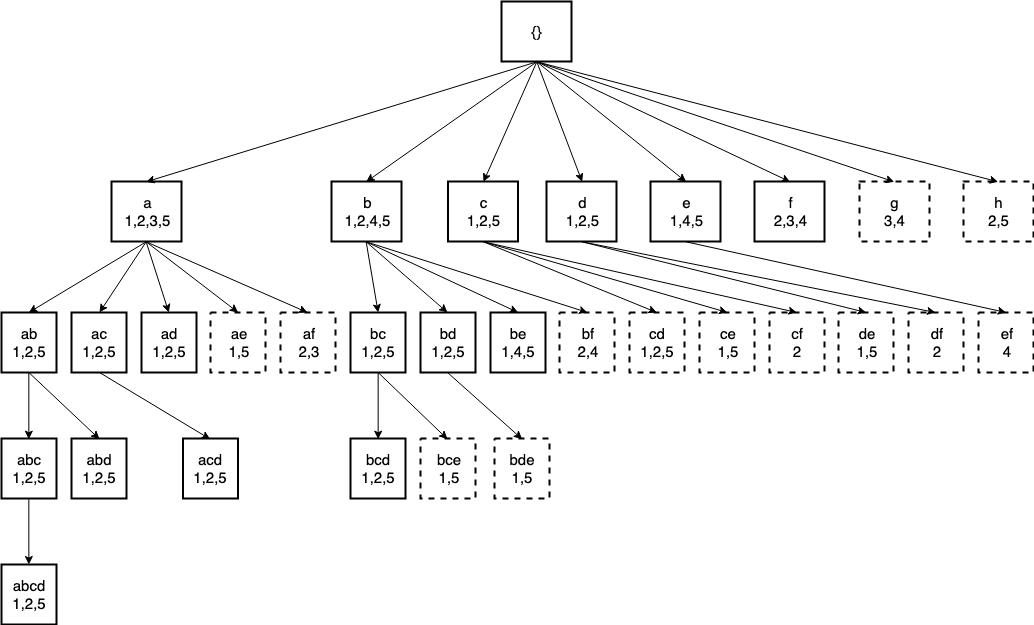
\includegraphics[width=1.0\textwidth]{RelatedWorks/eclat.png}
    \caption{An example of Eclat \cite{survey2014}}
    \label{fig:eclat}
\end{figure}

Another mainstream popular tree-based algorithm is FP-Tree. It uses compressed representations of the transactional database for more efficient counting.

\begin{definition}[\textbf{\textit{FP-Growth}}]
\label{FP}
The FP-Growth Algorithm, proposed by Han \cite{fp}, is an efficient and scalable method for mining the complete set of frequent patterns by pattern fragment growth, using an extended prefix-tree structure for storing compressed and crucial information about frequent patterns named frequent-pattern tree.
\end{definition}

In the first pass, the algorithm counts occurrence of items (attribute-value pairs) in the dataset, and stores them to 'header table'. In the second pass, it builds the FP-Tree structure by inserting instances. Items in each instance have to be sorted by descending order of their frequency in the dataset, so that the tree can be processed quickly. Items in each instance that do not meet minimum coverage threshold are discarded. If many instances share most frequent items, FP-Tree provides high compression close to tree root.

Now we can build an FP-Tree based on the support values of each distinct item in the Table \ref{tb:tidlist} which is illustrated in Figure \ref{fig:fp} \cite{survey2014}.

\begin{figure}[H]
    \centering
    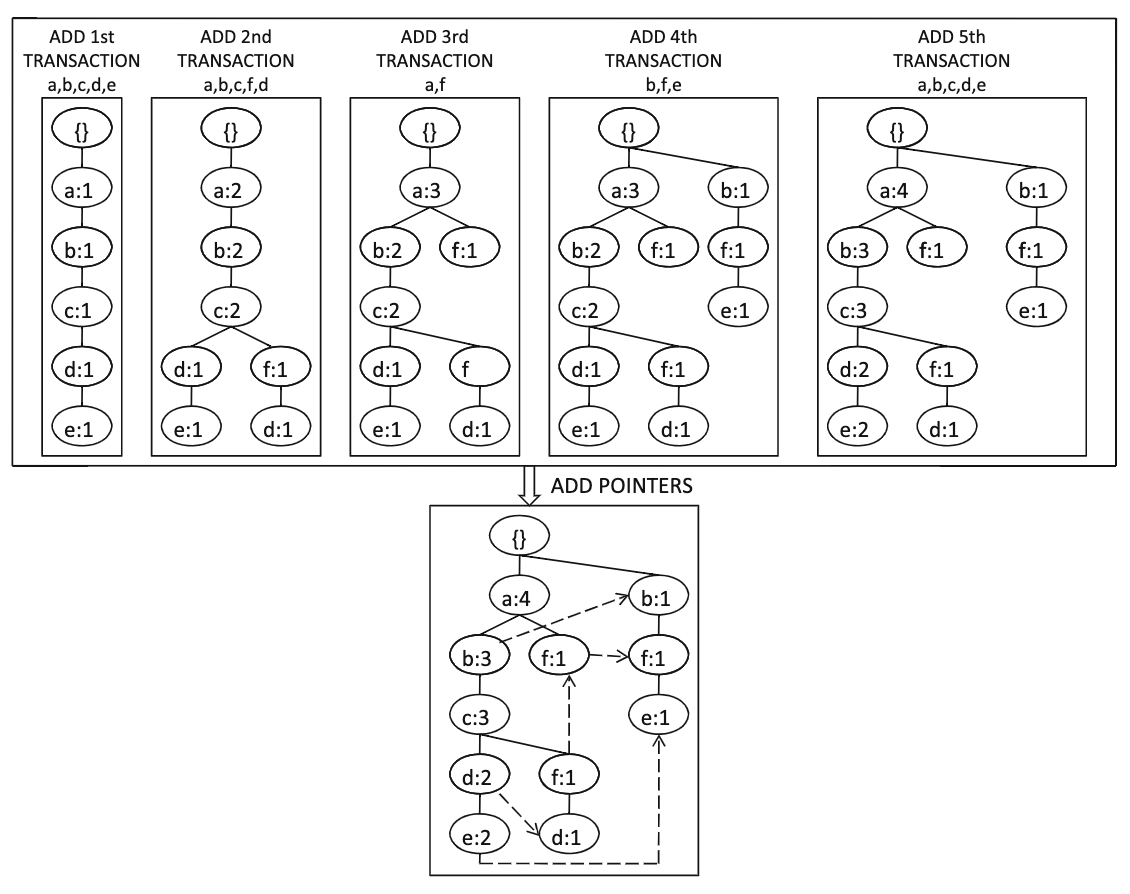
\includegraphics[width=1.0\textwidth]{RelatedWorks/fptree.png}
    \caption{An example of FP-Tree \cite{survey2014}}
    \label{fig:fp}
\end{figure}

When the situation becomes data stream mining, which means the data volume gets incredibly large, FP-Tree becomes very computational costly in both run time and space complexity. There are many existing researches \cite{fpopt1, fpopt2, fpopt3, fpopt4, fpopt5, fpopt6} focusing on tackling these issues. Most of the optimisations can be divided into two categories, one is using an advanced data structure to improve the performance like using arrays \cite{fpopt3}, another one holds partitioned database in the memory, for instance, CFP-Tree \cite{fpopt6}. Next, we are going to briefly discuss these two different mechanisms.

\begin{definition}[\textbf{\textit{CFP-Tree}}]
\label{ctpro}
Compact FP-Tree (CFP-Tree) was proposed by Sucahyo and Gopalan in 2004 \cite{fpopt6}. CFP-Tree is able to save the same amount information of FP-Tree but consumes 50\% memory. CFP-Tree does not have nodes that contains item label and support value, it maps item labels into index of thee head table - a sequence of integers. CPF-Tree accumulates duplicated sub-trees and keeps details in the leftmost branch, which achieves the compression of FP-Tree. 
\end{definition}

As FP-Tree constructs many conditional trees during the expansion, when the support value gets very low or association rule gets very long, it may gets beyond the system's affordability. CT-PRO algorithm solves this problem by adopting a non-recursive procedure. CT-PRO divides database into different parts which individual will be treated as a sole CFP-Tree independently. This significantly saves the memory use of the mining process.

To save the time for FP-growth to traverse FP-Tree, Grahne and Zhu \cite{fpopt3} used an array-like structure to improve FP-Tree. There are usually two traversals in the procedure of conducting FP-Tree, all frequent items are found during the first traversal and initialise a FP-Tree at the same time by finishing its header table construction. Then followed by the second traversal which will build a new tree. Grahne and Zhu \cite{fpopt3} started with creating an array during the first FP-Tree was construction to keep the information without the first scan.

This technique works significantly well when the database is very sparse. Sparse database requires more time for traversal which is massively reduced by using an array-like structure.

After all the discussions we had on association rule mining techniques, we may still need to get a rough idea of how data streams look alike before mining rules out from them. There are many algorithms been developed to construct a synopsis for data streams. One of the most important tasks is to get the top frequent items out from data streams.  

\subsection{Lossy Counting}

Lossy Counting \cite{lossy} provides a simple and efficient approximation for data stream to identify all elements whose current frequency exceeds a support threshold.

\begin{enumerate}
    \item First, divide data stream into fixed-sized windows.
    \item Second, increment the frequency count of each item according to the new window values. After each window, decrement all counters by 1.
    \item Last, repeat and update counters and after each window, decrement all counters by 1.
\end{enumerate}

In the end, the most frequently items will ``survive''. Given a frequency threshold $f$, a tolerance error $e$, and total number of elements $N$, all items with more than $f\times N - e \times N$ frequency will be returned as result. The primary window size is determined by the error rate $e$: $1/e$, and the number of windows will be $\lceil N\times e \rceil$, the worst case we need $(1/e)\times log(e\times N)$ counters.

\begin{figure}[H]
    \centering
    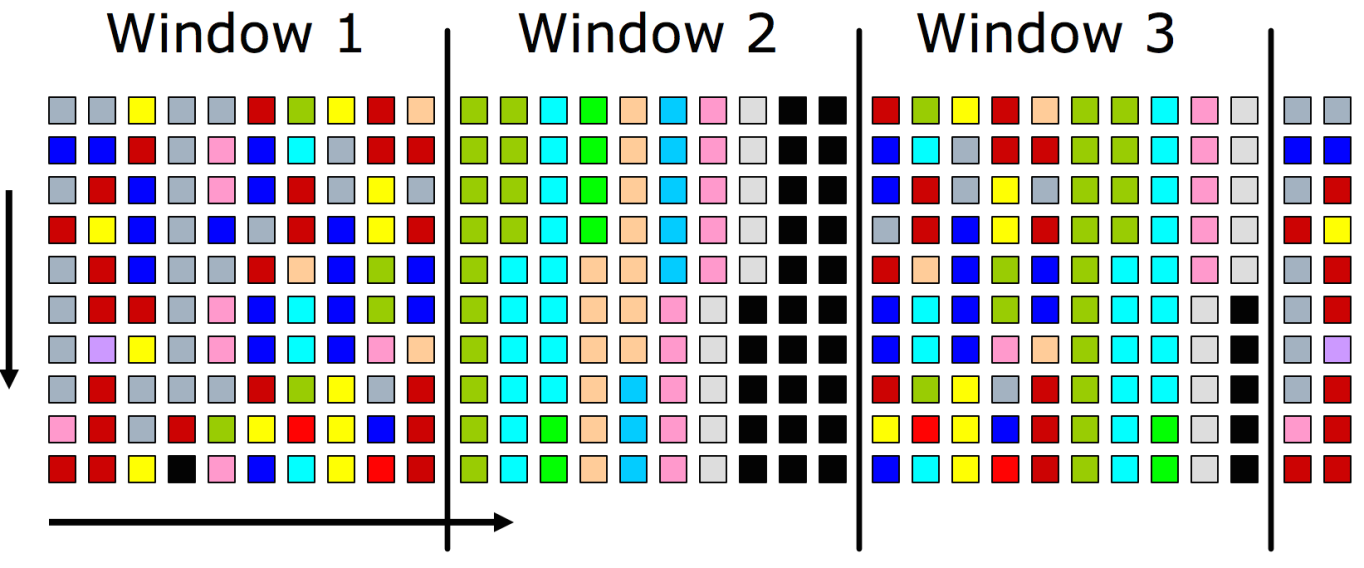
\includegraphics[width=0.8\textwidth]{RelatedWorks/lossy1.png}
    \caption{Step 1: divide windows \cite{lossymanku}}
    \label{fig:lossy1}
\end{figure}

\begin{figure}[H]
    \centering
    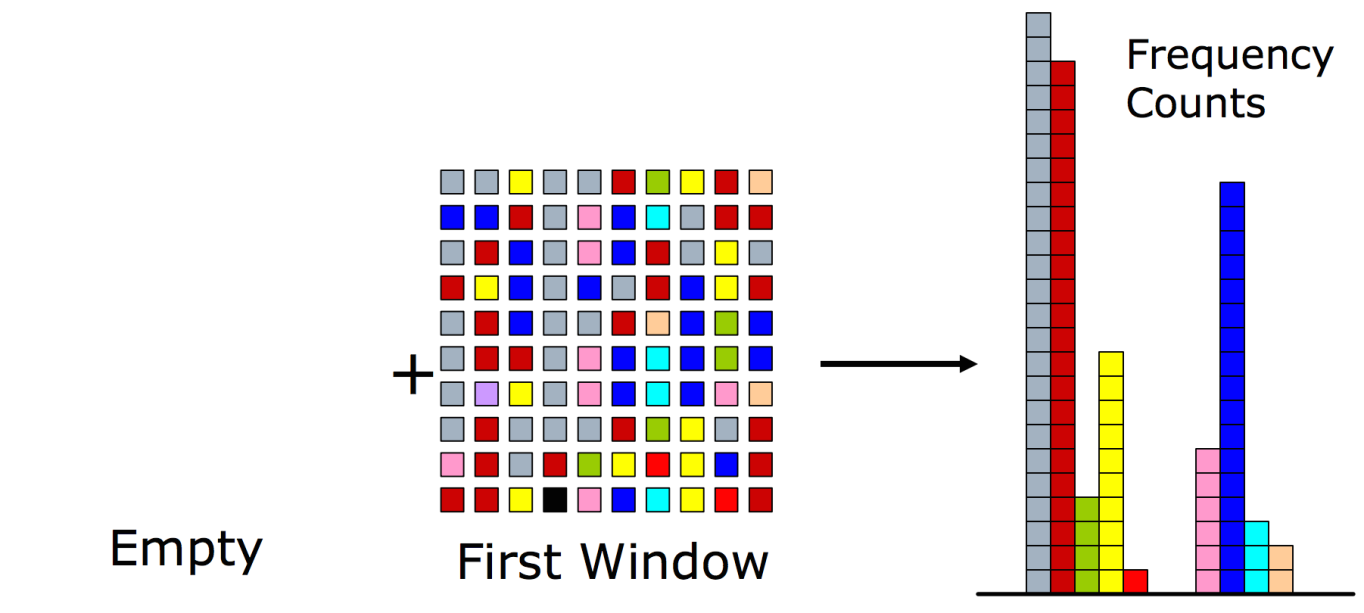
\includegraphics[width=0.8\textwidth]{RelatedWorks/lossy2.png}
    \caption{Step 2: increment counters \cite{lossymanku}}
    \label{fig:lossy2}
\end{figure}

\begin{figure}[H]
    \centering
    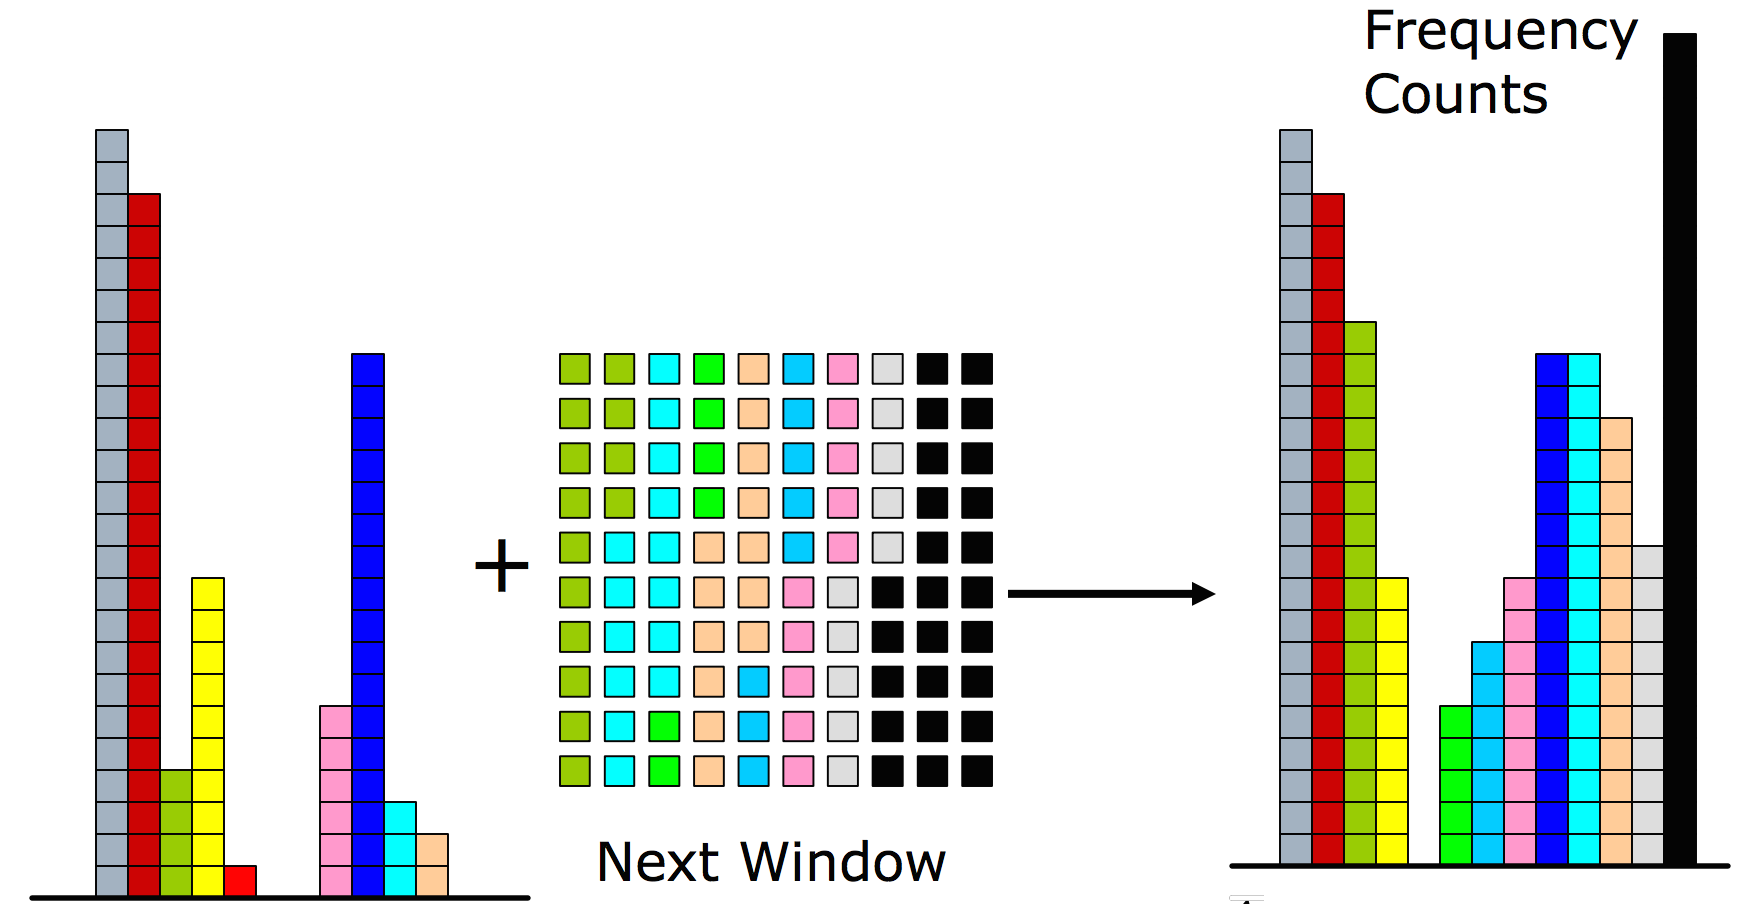
\includegraphics[width=0.8\textwidth]{RelatedWorks/lossy3.png}
    \caption{Step 3: decrement counters by 1 at boundary}
    \label{fig:lossy3}
\end{figure}



\subsection{Limitations of ``Support-Confidence” Framework}

Webb \cite{topk} pointed out that the traditional association rules mining techniques using minimum support and confidence threshold has numbers of limitations when apply them to most of the real-world scenarios.

First, there are some rare patterns which may be identified as frequent patterns by mistake. For instance, in the supermarket basket scenario, some terms may appear to be frequent but in fact, customers may act behalf of their company or friends which potentially lead to misclassifications.

Also, minimum support technique is relevantly a crude mechanism. It is almost impossible to pre-set a perfect minimum support threshold in advance, before the whole data stream is being analysed. Finding an appropriate threshold is usually tricky and sometimes leads to errors.

Dense data cannot be analysed by minimum support technique. It works fine when the terms in each transaction being relevantly infrequent. If numbers of terms appear frequently in each transaction, then the algorithm will produce a large number of interesting associations which is obviously wrong.

One of the most important, minimum support cannot be set low enough to
capture all valid rules. Nor can it be set high enough to exclude all spurious rules. Generally, minimum support may be irrelevant to the interestingness of associations.

\section{Concept Drift Mining} \label{sec:2.3}
This chapter focuses on concept drift detection, starts with definitions and types of concept drifts. Different kinds of drift detectors will also be discussed.

\subsection{Concept Drift}
Due to the inherent temporal aspect of data streams, the underlying data distribution of streams may change over time, known as concept drifts. Concept drift can make the machine learning model inaccurate because of the inconsistency between existing data and new data.

A transactional data stream $\mathcal{D}$ with $n$ elements $\mathcal{D} = \{T_1, T_2, ..., T_n\}$ where by $T_i$ represents a transaction at time $i$. At the time point $t$, let \mathcal{D}_1=(T_1, T_2, ..., T_t)$, $\mathcal{D}_2=(T_t_+_1, T_t_+_2, ..., T_n)$ be two instance of $\mathcal{D}$, with $0<t<n$ and their mean $\mu_1$ and $\mu_2$ respectively.

\begin{definition}[\textbf{\textit{Concept Drift Detection Problem}}]
\label{conceptdrift}
The concept drift detection problem is a statistical hypothesis test with the null hypothesis $H_0$ that $\mu_1=\mu_2$ and the alternative hypothesis $H_A$, that is, $\mu_1\neq\mu_2$.
\end{definition}

If the two samples $\mathcal{D}_1$ and $\mathcal{D}_2$ are drawn from the same distribution, the null hypothesis $H_0$ is justified, otherwise, the alternative hypothesis $H_A$ is accepted, a concept drift has been detected at the time point $t+1$. The position of this certain time point is also called \textit{drift point}.

In the data stream mining task, a concept drift may occur in different forms. In the next section, we review the types of concept drifts that can occur during data streams.

\subsection{Types of Concept Drifts}
Concept drifts can happen in different forms, there are two common types of drifts: abrupt drift and gradual drift.

\begin{definition}[\textbf{\textit{Abrupt Drift}}]
\label{abruptdrift}
An abrupt drift happens when there is a change in underlying distribution occurs instantaneously. Once an abrupt drift is detected, it usually means the whole distribution will remain changed after that point. 
\end{definition}
The figure below illustrates a simple example of an abrupt drift.

\begin{figure}[h!]
    \centering
    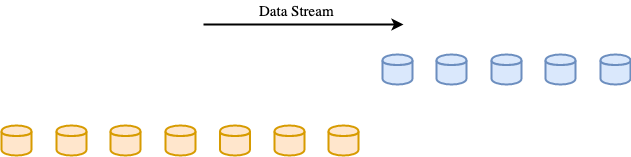
\includegraphics[width=0.7\textwidth]{RelatedWorks/abrupt.png}
    \caption{An example of abrupt drift}
    \label{fig:abrupt}
\end{figure}

%\paragraph{Gradual drift}\mbox{}\\

\begin{definition}[\textbf{\textit{Gradual Drift}}]
\label{gradualdrift}
Gradual drift, also known as incremental drift, is different from an abrupt drift. While abrupt change is caused by distribution changes instantaneously, gradual drift happens incrementally. This means between a potential change happens and the whole distribution actually changes, the data stream may remain the similar distribution as original.
\end{definition}

A simple example of an gradual drift has been illustrated below.

\begin{figure}[h!]
    \centering
    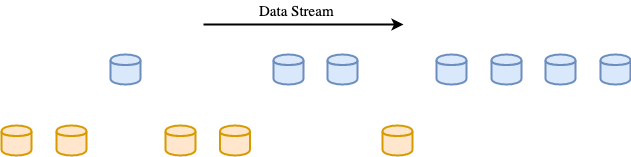
\includegraphics[width=0.7\textwidth]{RelatedWorks/gradual.png}
    \caption{An example of gradual drift}
    \label{fig:gradual}
\end{figure}

\subsection{Regional Concept Drift}%\mbox{}\\
Most distribution based drift detection methods assume that a drift occurs abruptly at a time point, incrementally, or gradually in a time period \cite{gradual}. As a result, the split time point between old and new concepts is the key solution. However, this time-oriented ``one-cut" process could not adapt to the real-world scenarios well. Accordingly, the data arrived before that drift point is discarded. Thus, if a drift only occurs in a small region of the entire feature space, the other non-drifted regions may also be suspended, thereby reducing the learning efficiency of models. %To retrieve non-drifted information from suspended historical data, similar to the buffer system \cite{buffer} used to find the best drift time point to identify concepts, we proposed a simple solution to identify regional drifts and integrate it into our self-sufficient itemset mining process.

\begin{figure}[h!]
    \centering
    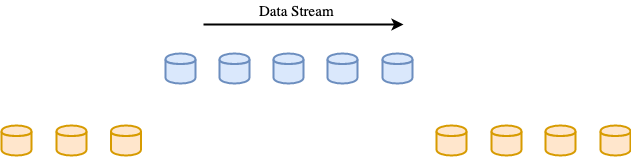
\includegraphics[width=0.7\textwidth]{RelatedWorks/regional.png}
    \caption{An example of regional drift}
    \label{fig:gradual}
\end{figure}

\subsection{Drift Detectors}

%\paragraph{DDM}\mbox{}\\

\begin{definition}[\textbf{\textit{DDM}}]
\label{ddm}
Drift Detection Method (DDM) is one of the earliest proposed drift detectors. DDM was built based on the PAC learning model premise, it assumes that the error rate decreases with more examples when the distribution is stationary.
\end{definition}

DDM analyses the error rate and some statistics such as standard deviation. There are normally two preset threshold: change and warning. When DDM detects an increase in the error rate and it surpasses the change threshold, a drift will be detected and reported. If the increase does not surpass the change threshold but the warning threshold, DDM will report a warning zone which indicates there might be changes happening in the near future.

%\paragraph{EDDM}\mbox{}\\
\begin{definition}[\textbf{\textit{EDDM}}]
\label{eddm}
%Drift Detection Method (DDM) has been proved useful for abrupt change detection. 
To improve the accuracy of detecting gradual changes in data stream, Early Drift Detection Method (EDDM) was proposed by keeping track of the average distance between two errors instead of only the error rate. 
\end{definition}

Similar to DMM, EDDM also has warning and change thresholds which are used for determine change levels.

%\paragraph{Page Hinkley}\mbox{}\\
\begin{definition}[\textbf{\textit{Page Hinkley}}]
\label{ph}

Page Hinkley \cite{PHT} method works by computing the observed values and their mean up to the current moment. 
\end{definition}

Page Hinkley won't output warning zone warnings, only change detection. The method works by means of the Page Hinkley test. Page Hinkley Test works as a sequential analysis mechanism which is often used as a concept drift detector. In general lines it will detect a concept drift if the observed mean at some instant is greater then a threshold value lambda \cite{PHT}.

%\paragraph{ADWIN}\mbox{}\\
\begin{definition}[\textbf{\textit{ADWIN}}]
\label{adwin}
ADWIN stands for ADaptive WINdowing, is an adaptive sliding window algorithm for detecting change, and keeping updated statistics about a data stream. 
\end{definition}

ADWIN decides the size of the window by cutting the statistics' window at different points and analysing the average of some statistic over these two windows. If the absolute value of the difference between the two averages surpasses a pre-defined threshold, change is detected at that point and all data before that time is discarded. 

ADWIN guarantees rigorous performance, by bounding its false positive and negative rates, which makes it an ideal solution for high-precision required situations.


\section{Self-Sufficient Itemsets} \label{sec:2.4}
While there are large amounts of literature on identifying and discovering association rules \cite{arm1,arm2,arm3,arm4}), they are all heavily reliant on using a support threshold to derive interesting association rules. The existing literature on identifying and discovering interesting rules beyond using support or frequency of occurrence is relatively sparse. Webb~\cite{patternwebb} points out that many pattern mining algorithms suffer from type-I errors which usually identifies infrequent itemsets as frequent. To deal with the drawbacks of the pure ``support-confidence" framework for pattern mining, Hamalainen \cite{kingfisher} proposed a solution which handles non-monotonicity. It also prunes redundant rules on-line. The quality of rules is estimated by the Fisher's exact test. `Self-sufficient itemsets" \cite{ssi} were created to solve this dilemma by contributing a set of constraints and statistical tests that can be applied during and after itemset discovery to identify itemsets whose frequency cannot be explained solely by either higher or lower-order interactions between factors within the data.

To improve the pure ``support-confidence” framework, Webb \cite{ssi} defined self-sufficient itemsets, which proposed \textit{itemset leverage}. \emph{Itemset leverage} is a measure for the degree of potential interest that arises naturally from the tests developed in \cite{ssi} by checking their productivity and non-redundancy. We further adapted the method by using Fisher's exact test to check for the minimum support threshold as well. This has been used in previous techniques \cite{kingfisher,ssi}.%[].

To be self-sufficient, an itemset must be \textit{productive}, \textit{non-redundant} and \textit{independently productive}.

Firstly, we introduce the definition of cover, similar to support, which helps us understand how self-sufficient itemset.

\begin{definition}[\textbf{\textit{Cover}}]
\label{df:cover}
The \textit{cover} of an itemset $x$ is the set of TIDs which contains $x$:
\end{definition}

\begin{equation}
\label{eq:cover}
cov(x, \mathcal{D}) = \{i: 1\leq i\leq |\mathcal{D}| \wedge x \subseteq \mathcal{D}_i\}
\end{equation}

\begin{definition}[\textbf{\textit{Fisher's exact test}}]
\label{df:fishers}
Fisher's exact test is the main statistical test used to define self-sufficient itemset. It is a statistical test used to determine if there are nonrandom associations between two categorical variables.

Let there exist two such variables $X$ and $Y$, with $m$ and $n$ observed states, respectively. Now form an $m\times n$ matrix in which the entries $a_i_j$ represent the number of observations in which $x = i$ and $y = j$. Calculate the row and column sums $R_i$ and $C_j$, respectively, and the total sum: 

\begin{equation}
\label{eq:fisherssum}
N = \sum_{i} R_i = \sum_{j} C_j
\end{equation}

of the matrix. Then calculate the conditional probability of getting the actual matrix given the particular row and column sums, given by:

\begin{equation}
\label{eq:fishersformula}
P_{cutoff}=\frac{(R_1! R_2! \cdots R_m!)(C_1! C_2! \cdots C_n!)}{N!\prod_{i,j} a_{ij}!}
\end{equation}

which is a multivariate generalisation of the hyper-geometric probability function. Now find all possible matrices of non-negative integers consistent with the row and column sums $R_i$ and $C_j$. For each one, calculate the associated conditional probability using Eq. \ref{eq:fishersformula}, where the sum of these probabilities must be 1.
\end{definition}


\begin{definition}[\textbf{\textit{Productivity}}]
\label{df:productivity}
An itemset has to satisfy the following condition to be self-sufficient: any partition of it into two subsets of terms must be positively correlated with each other.

\begin{equation}
\label{productive}
P(R \supseteq x) >  \underset{y \subsetneq x}{max}(P(R \supseteq y)P(R \supseteq x \setminus y))
\end{equation}

It is hard to obtain the probabilities which leads us to perform a statistical test. In this case, Fisher's Exact Test is being used. The $p$-value for the case whether itemset $x$ and $y$ of dataset $D$ are positively correlated should look like this:

\begin{equation}
\label{fishersp}
p_{F}(x, y, D) = \sum_{i=0}^{\omega} \frac{\binom{\#(x, D)}{\#(x, y, D)+i}\binom{\#(\neg x, D)}{\#(\neg x, y, D)+i}}{\binom{n}{\#(y, D)}}
\end{equation}

where $\omega$ = min($\#(x,\neg y, D), \#(\neg x, \neg y, D)$). \cite{ssi}

To test productivity for an itemset $m$ , all of its partitions need to be passed the Fisher's test.

\begin{equation}
\label{fisherspartition}
p(m,D) = \underset{x \subsetneq m}{max}(p(x, m \setminus x, D))
\end{equation}


\end{definition}


\begin{definition}[\textbf{\textit{Redundancy}}]
\label{df:redundancy}
Redundancy test provides another criteria to filter itemsets that are unlikely to be interesting. If an itemset $x$ has a subset $y$ which contains an item $i$ that subsumes $y\setminus i$, we define $x$ as redundant. This has also been discussed for constraints of association rule mining. \cite{redundant}

\begin{equation}
\label{eq:redundant}
\exists i, y : i\in y \wedge y \subsetneq x \wedge cov(\{i\}) \supseteq cov(y \setminus i)
\end{equation}

\end{definition}


\begin{definition}[\textbf{\textit{Independent Productivity}}]
\label{df:indprod}
In terms of quantifying interestingness, the Min Partition Measure (MPM) is used. Webb \cite{ssi} suggests that itemset measures should be developed from a rule measure by selecting the least extreme value that results from applying the measure to any rule that can be created by partitioning the itemset $x$ into an antecedent $y$ and consequent $z = x \setminus y$. In this work, two measures: $leverage, \delta$ and $lift, \gamma$ have been used as the formulas Eq. \ref{eq:leverage} and Eq. \ref{eq:lift} illustrated below:

\begin{equation}
\label{eq:leverage}
\delta(x) = \underset{y \subsetneq x}{min}(sup(x)-sup(y)\times sup(x \setminus y))
\end{equation}

\begin{equation}
\label{eq:lift}
\gamma(x) = \underset{y \subsetneq x}{min}(sup(x)/ [sup(y)\times sup(x \setminus y)])
\end{equation}

\end{definition}

\subsection{OPUSMiner}
OPUSMiner~\cite{patternwebb} is developed to find the top-$k$ productive, non-redundant itemsets from transaction data. The OPUS Miner algorithm uses the OPUS search algorithm to efficiently discover the key associations in transaction data, in the form of self-sufficient itemsets, using either $leverage, \delta$ as in Eq. \ref{eq:leverage} or $lift, \gamma$ as in Eq. \ref{eq:lift}.

OPUSMiner is conducted with four parts: expandItemset, checkPartitions, checkImmediateSubsets and checkIndeproductive. Each part will achive the cooresponding task which is a compulsory condition for an itemset to be self-sufficient.

\begin{enumerate}
    \item expandItemset: explore all supersets of a generated itemset $X$ from beginning by adding items in the frequent item list $q$.
    \item checkPartitions: check the binary partitions of itemset $X$. Return the minimum value of $\delta $ and $ \gamma$ and the maximum $p$-value $p$ with respect to any partition.
    \item checkImmediateSubsets: check all subsets of $X$ formed by removing a single item to determine whether $X$ fails the Apriori test and whether supersets of $X$ must fail either the Apriori or redundancy test.
    \item checkIndeproductive: post-process the top $k$ itemsets to determine whether they are independently-productive.
\end{enumerate}

OPUS Miner systematically traverses viable regions of the search space, maintaining a collection of the top-$k$ productive non-redundant itemsets in the search space explored. When all of the viable regions have been explored, the top-$k$ productive non-redundant itemsets in the search space explored must be the top-$k$ for the entire search space.

\subsection{Concept Drifts in Self-Sufficient Itemsets Mining}

According to \cite{classsurvey}, an important problem in the streaming scenario is classification, where data is labelled into categories or classes. As data streams are considered to be non-stationary, the distribution of data and their class labels will likely change over time. Concept drift detection methods are used to monitor classification errors from classifiers (with binary input where 0 is a correct classification and 1 is a misclassification) to identify when changes happen. In our scenario, we want to determine how frequent potential ‘interesting’ itemsets occur in the data stream. The measure we used to feed our drift detector with will be the binary occurrence of itemsets in each transaction of the data stream (0 if itemset is not present and 1 if itemset is present). Gama et al. \cite{driftsurvey} gives an overview of mainstream drift detectors used for data stream. One of the most widely used detector is ADWIN \cite{adwin}. ADWIN detects concept drifts using an adaptive windowing strategy and signals drifts if the absolute value of the difference between any two windows surpasses a pre-defined threshold, derived from Hoeffding Bound.

\section{Summary of Literature} \label{sec:2.5}

There are many researches focusing on the field of association rule mining and concept drift mining. We reviewed the research problems and studies their proposed solutions and methodologies.

In association rule mining, the major problem is to discover significant patterns out from unlabelled item based data which usually comes in a form of transaction, as known as transactional data stream using unsupervised machine learning techniques. Traditional ``support-confidence'' framework like Apriori \cite{apriori} and FP-growth \cite{fp} has been adopted to solve most of the association rule mining problems in the past decades, its drawbacks has become an issue for association rule mining. We reviewed several new association rule mining algorithms proposed to solve these drawbacks such as improving the adaptability of support threshold \cite{armlin}, adding statistical tests to filter rules \cite{kingfisher} and defining new restraints to create association rules \cite{topk,ssi}. 

Concept drift mining focuses on detecting the underlying distribution change and adapting to the drifts detected. Drifts have different types such as abrupt, gradual and regional drifts. The difference between abrupt and gradual drifts is the time they occur: abrupt drifts only happen in a very short period or time while gradual drifts may need longer period. Regional drifts are those drifts which occur during a specific period of time. Many concept drift detectors have been proposed to solve the problem, we have reviewed them in different categories in statistics control (e.g. EDDM and DDM), sequential analysis (e.g. Page Hinkley), and sliding-window monitoring (e.g. ADWIN).




\chapter{Self-Sufficient Itemset Stream Mining}
\label{chapt:ASSIM}
Our earlier chapters have introduced definitions and problems that target mining interesting association rule from unlabelled data streams where data is transactional item-based using unsupervised learning. In this chapter, we focus on how to discover self-sufficient itemsets from unlabelled data streams.

There has been some research in the area of interesting association rule mining where researchers try to capture patterns involving events that happens frequently or appear in a certain pattern in a static dataset. Although much of the research focus in using ``support-confidence'' framework on finding association rule, self-sufficient are shown to be more accurate and adaptive by using several statistical tests. Until now, most of the research on this area concentrates only on finding self-sufficient itemsets in a static dataset. With the proliferation of applications which generate data streams, such as network logs and banking transactions, applying techniques that mine from static datasets onto dynamic data streams is not practical. In this chapter, we address the research problem of mining self-sufficient itemsets from dynamic data streams and propose an adaptive approach.

The main contributions of this chapter are:
\begin{itemize}
\item We propose a novel approach called  Adaptive self-sufficient Itemset Miner (ASSIM), which facilitates discovery of self-sufficient itemsets in a data stream environment with regional drift detection.
\item With ASSIM we discuss the idea of using a sliding window to achieve actual online learning for data stream rather than batch processing.
\end{itemize}

\section{Adaptive Self-Sufficient Itemset Miner (ASSIM)}
%What does ASSIM do? 
To mine self-sufficient itemsets and to solve the regional concept drift problem at the same time, we propose a new technique: Adaptive self-sufficient Itemset Miner (ASSIM). ASSIM is able to mine self-sufficient itemsets in an online mode, and at the same time, detect regional drifts among generated self-sufficient itemsets and adapt the drifts to the self-sufficient itemset generation process.

%Why do we need ASSIM?
The current self-sufficient miner \cite{ssi} is designed for static databases. To use this technique unaltered on a data stream has its pitfalls. This includes regional concept drifts that may occur over time in data stream, making previously generated self-sufficient itemsets inaccurate. We can adapt self-sufficient miner by generating itemsets at fixed intervals but this is inefficient, and there may be a delay between when changes happen in the data stream to when the new set of itemsets are generated. Another possibility is that if the intervals are set too far apart we may miss out on generating those itemsets all together. Our framework is designed to overcome this problem.


\begin{figure}[h!]
    \centering
\tikzstyle{decision} = [diamond, draw, fill=blue!20, 
    text width=4.5em, text badly centered, node distance=3cm, inner sep=0pt]
\tikzstyle{block} = [rectangle, draw, fill=blue!20, 
    text width=8em, text centerd, rounded corners, minimum height=4em]
\tikzstyle{line} = [draw, -latex']
\tikzstyle{cloud} = [draw, ellipse,fill=red!20, node distance=5cm,
    minimum height=4em]

\resizebox {\columnwidth} {!} {
\begin{tikzpicture}[node distance = 4cm, auto]
Bass
    \node [block] (init) {Batch Size Calculator};
    \node [cloud, left of=init] (data) {$D = T_1, T_2, \ldots T_n$};
    \node[above of = data,node distance=1cm]{Input (Data Stream)};
    \node [block, right of=init] (system) {Self-sufficient Itemset Generator};
    \node [block, right of=system] (rcda) {Regional\\ Concept Drift Adaptor (RCDA)};
    \node[cloud, right of = rcda](SSI){Self-sufficient Itemsets};
    % Draw edges
    \path [line] (data.east) |-(init);
    \path [line] (init) |- (system);
    \path [line] (system) |- (rcda);
    
    \path[line, dashed] (rcda.south) -| ([xshift=0cm, yshift=-1cm]rcda.south) -- ([xshift=0cm, yshift=-1cm]system.south) |- (system.south);
    \path[line](rcda.east) |- (SSI);
\end{tikzpicture}
}
    \caption{Framework of Adaptive Self-sufficient Itemset Miner }
    \label{fig:ASSIM}
\end{figure} 


An illustration our ASSIM framework is shown in Fig. \ref{fig:ASSIM}. It gives a general idea of the structure of ASSIM and how the data flows inside ASSIM.
As transactions are fed into ASSIM, they will be processed first in the Batch Size Calculator (BSC) to get an appropriate batch size before we enter the itemset mining process. The calculation of the batch size is crucial to avoid over-fitting. We realised that there are possible minor fluctuations within a data streams. Thus, a stable bucket allows for a more representative sample to be used in the mining process.   

Using the calculated batch size, the self-sufficient Itemset Generator (SSIG) can be used to generate self-sufficient itemsets. All generated self-sufficient itemsets will be checked for potential regional concept drifts by the Regional Concept Drift Adaptor (RCDA). Once a regional drift has been detected, RCDA will check the drift type and determine whether SSIG needs to generate new self-sufficient itemsets from the drift point or not.

Our Adaptive Self-Sufficient Itemset Miner algorithm is shown in Algorithm \ref{alg:assim}, which presents the top level of the technique and how its parts interact with each other.

\begin{algorithm}[h!]
\caption{Adaptive Self-Sufficient Itemset Miner (ASSIM)} 
\label{alg:assim}
\hspace*{0.02in} {\bf Input:} 
data stream $\mathcal{D}$ of transactions $\{T_1, ..., T_n\}$, $k$\\
\hspace*{0.02in} {\bf Output:} 
\textit{result}(set of self-sufficient itemsets: $S$);
\begin{algorithmic}[1]

\While{exist($\mathcal{D}$)} 
  \State $frequentItems\leftarrow$ BSC($\mathcal{D}$)
  \State stable batches $\leftarrow$ BSC($\mathcal{D}$)
  \State $S\leftarrow$ SSIG($k$, \textit{frequentItems});
  \State RCDA($S:\{s_1, ..., s_m$\}, $\mathcal{D}$: $\{T_1, ..., T_n\}$)
  \State $S'\leftarrow$ RCDA($S, \mathcal{D}$)
  \State $S \leftarrow S + S'$
\EndWhile

\State \Return set of self-sufficient itemsets $S$
\end{algorithmic}
\end{algorithm}

\section{Batch Processing}

%What does Batch Size Calculator (BSC) do?

The Batch Size Calculator (BSC) is the first part of our ASSIM framework. It was designed to handle frequency counting and batch size calculation. It provides an approximation of items’ frequencies. The main purpose of this is to ensure that a proper stable batch size was used before we mined for self-sufficient itemsets. As with any data streams, selecting an adequate learning window is essential to ensure the quality of the results produced. If the batch size is too small, the variance of the itemsets produced may be an issue. If the batch size is too large, then there is a lag or time delay between when transactions happen to when it is mined.  

%Why do we need BSC?
Data stream mining requires a stable and comparable batch size to represent the current state. In this case, Lossy Counting \cite{lossy} has been used because of its low computational cost which improves both memory and run-time processing. As only an approximated ranking list is needed, for the expansion process we used Lossy Counting. To use Lossy counting, we divide the incoming data stream into buckets. We keep a running histogram of the unique items for each transaction in the data stream. If items appear in a transaction within a bucket size, we increment the frequency count of those items. At the end of each bucket, we decrement each of the counters by 1. At the end, the most frequently viewed items `survive'.

%How does BSC works?

\subsection{Stable Batch Size}

A data stream of items $\{x_1, x_2, x_3, \C, x_m\}^{(t)}$ are the inputs at time $t$ to BSC, whereby $m$ is the number of unique items. Their frequencies will be calculated using Lossy Counting, and generate a list of top $n$ frequent items $\{a_1, a_2, \ldots, a_n\}^{(t)}$. Meanwhile, in order to calculate a stable and comparable batch size for the self-sufficient Itemset Generator, the distribution of each frequent items $D^{(t)} = \{d_a__1,$ $d_a__2$, \ldots, $d_a__n$ $\}^{(t)}$ in each Lossy Counting bucket will be calculated and compared with the prior bucket of $D^{(t-b)}= \{d_a__1,$ $ d_a__2$, \ldots, $d_a__n$ $\}^{(t-b)}$, where $b$ is the bucket size. 

When a new bucket has been processed, we average the frequency differences of top $k$ frequent items (picked from Lossy Counting) between the current bucket and the prior one. If the average frequency difference is larger than threshold $\tau$, 
\[
\frac{1}{k}\sum d_a_k^{(t)} - \frac{1}{k}\sum d_a_k^{(t-b)} > \tau,
\]   
we report the bucket number $B$ and the first batch size will be $B \times (1/e)$ whereby $e$ is the tolerance error rate for the approximation.

Our Batch Size Calculator algorithm is shown in Algorithm \ref{alg:bsc}.

\begin{algorithm}[h!]
\caption{Batch Size Calculator (BSC)} 
\label{alg:bsc}
\hspace*{0.02in} {\bf Input:} 
data stream $\mathcal{D}$, threshold $\tau$, tolerance error rate $e$;\\
\hspace*{0.02in} {\bf Output:} 
\textit{batchSize}, \textit{result}(set of stable batches);
\begin{algorithmic}[1]

\While{exist($\mathcal{D}$)} 
  \State lossyCounting($\mathcal{D}$);
  \State \textit{frequentItems} $\{a_1,a_2,...,a_n\}\leftarrow$ result from lossyCounting;
  \State \textit{bucketSize} $b\leftarrow1/e$;
  \State $D^{(t)} = \{d_a__1,$ $d_a__2$, \ldots, $d_a__n$ $\}^{(t)}\leftarrow$ distribution of each frequent item in a bucket;
  \State compare $D^{(t-b)}$ with $D^{(t)}$;
  \If{average frequency difference $> \tau$}
      \State report the current bucket number $B$;
      \State \textit{batchSize} $\leftarrow B \times (1/e)$;
  \EndIf
\EndWhile

\State \Return set of stable batches
\end{algorithmic}
\end{algorithm}

\paragraph{An Example of BSC}

Given the dataset in Table \ref{tb:tid}, we show how stable batches  built using BSC. Table \ref{tb:fq} lists the items which have more than 30\% support in the dataset, which are used for calculating stable batches in Figure \ref{fig:bsc}. In this example, threshold $\tau$ is set to 25\%, tolerance error rate $e = 1/3$.

\begin{table}[h!]
\caption{Set of Transactions in 4 Buckets Each with Length 3}
\label{tb:tid}
\centering
 \begin{tabular}{p{4cm} p{4cm}} 
 \hline\hline
 \multicolumn{2}{c}{Transactions (tid: items)}\\
 \hline
 1: a, g h & 7: g \\ 
 %\hline
 2: a, g, h, i & 8: c, h \\
 %\hline
 3: b, c, d, f & 9: c, d, h \\
 %\hline
 4: b, d, j & 10: b, f \\
 %\hline
 5: c, f, h & 11: a, h  \\
 %\hline
 6: a, e, g, h & 12: a \\
 \hline
\end{tabular}
\end{table}

\begin{table}[h!]
\caption{Frequent Items with Frequencies}
\label{tb:fq}
\centering
 \begin{tabular}{p{4cm} p{4cm}} 
 \hline\hline
 \multicolumn{2}{c}{Frequent Items (item: frequency)}\\
 \hline
 h: 6 & g: 4\\
 %\hline
 a: 5 & c: 4\\
 \hline
\end{tabular}
\end{table}

Figure \ref{fig:bsc} illustrates the process of stable batch size calculation. It monitors the distribution differences between Lossy Counting buckets. In this example, frequency difference between Bucket 3 and Bucket 4 is 50\% which is over $\tau = 25\%$, so the number 3 will be report to divide batches. The first stable batch will have a size $3 \times 1/e = 9$.

\begin{figure}[H]
\caption{Distribution difference calculation}
\label{fig:bsc}
\centering
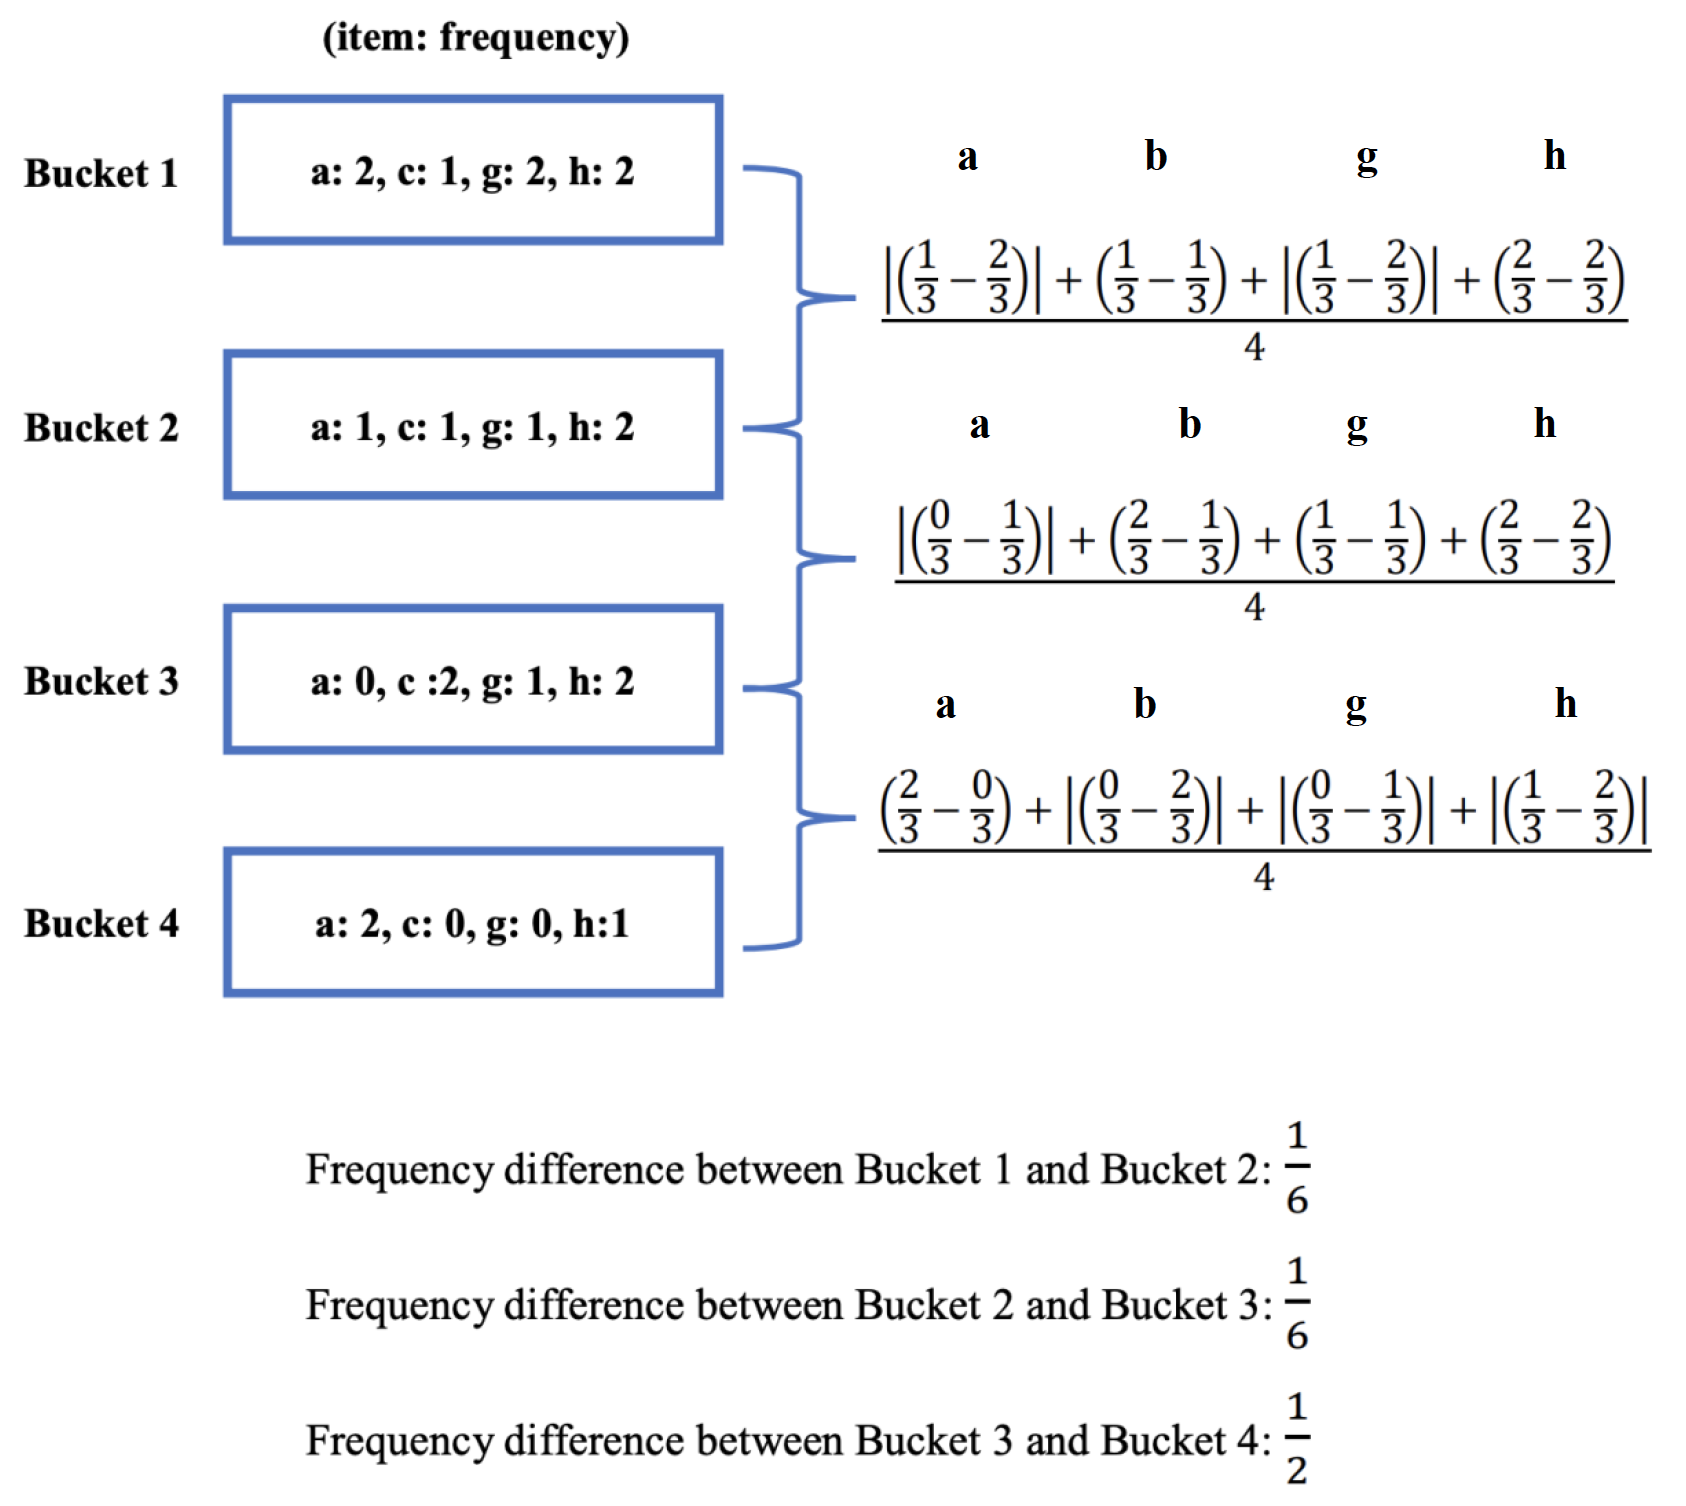
\includegraphics[scale=0.5]{Methodology/bsc.png}
\end{figure}

\section{Self-Sufficient Itemset Generation}
%What does this generator do?
We adapted the OPUS Miner proposed by Webb \cite{ssi}, for a dynamic streaming data. For a user-specified $k$ ($k=100$ by default) and interest measure, OPUS Miner find the top-$k$ productive non-redundant itemsets (as known as self-sufficient itemsets).

The original algorithm establishes a queue of items ordered in descending order on the upper bound on the value of any itemset that can include the item. However, one particular constraint with data stream algorithms is that there is only a one or limited pass through the data stream capability. This means the ability to run through an re-order of information is limited. In our self-sufficient Itemset Generator technique, we used the frequency counts from BSC to order the items instead. 
%Why we use this?

BSC provides an approximation of frequency counts for items, which helps us replace the static counting algorithm used in the original SSIG. The mining of the itemsets remains unmodified from the original version. 

%How does it work?

Our Self-Sufficient Itemset Generator algorithm is shown in Algorithm \ref{alg:ssig}.

\begin{algorithm}[h!]
\caption{Self-Sufficient Itemset Generator (SSIG)} 
\label{alg:ssig}
\hspace*{0.02in} {\bf Input:} 
$k$, \textit{frequentItems};\\
\hspace*{0.02in} {\bf Output:} 
\textit{result}($S$: set of self-sufficient itemsets);
\begin{algorithmic}[1]
\State OPUSMiner($k$, \textit{frequentItems})
\State $S \leftarrow$ result from OPUSMiner($k$, \textit{frequentItems})

\State \Return $S$: set of self-sufficient itemsets
\end{algorithmic}
\end{algorithm}


SSIG uses the list of frequent items obtain from BSC. We check for their interestingness and start to expand them into potential self-sufficient itemsets. Each newly generated itemsets and their partitions will be passed into SSIG to check for productivity and non-redundancy. Finally, all itemsets that passes the aforementioned constraints are considered as self-sufficient itemsets, $S$.

\begin{table}[H]
\caption{Set of 18 Transactions for SSIG}
\label{tb:tidlong}
\centering
 \begin{tabular}{p{4cm} p{4cm} p{4cm}}
 \hline\hline
 \multicolumn{3}{c}{Transactions (tid: items)}\\
 \hline
 1: a, g, h & 7: g & 13: a, c, h\\ 
 %\hline
 2: a, g, h, i & 8: c, h & 14: e, f, g\\
 %\hline
 3: b, c, d, f & 9: c, d, h & 15: a, b, e, h\\
 %\hline
 4: b, d, j & 10: b, f & 16: d, e, h\\
 %\hline
 5: c, f, h & 11: a, h & 17: a, e, g\\
 %\hline
 6: a, e, g, h & 12: a & 18: a, d, e, h\\
 \hline
\end{tabular}
\end{table}

\paragraph{An Example of SSIG}

Use the given dataset above in Table \ref{tb:tid}, we extended 6 more transactions for better mining result: Table \ref{tb:tidlong}. In this example, we will feed the following 18 transactions to SSIG to mine self-sufficient itemsets.

The mined self-sufficient itemsets from are $\{a, e\}, \{c, h\}$, and $\{e, h\}$.


\section{Regional Concept Drift Adaption}
%What does the RCDA do?
To retrieve non-drifted information from suspended historical data, similar to the buffer system \cite{buffer} used to find the best drift time point to identify concepts, we proposed a simple solution to identify regional drifts and integrate it into our self-sufficient itemset mining process.

The Regional Concept Drift Adaptor (RCDA) plays a key role in our ASSIM framework. It detects regional concept drifts in the generated self-sufficient itemsets. It analyses concept drifts and make decisions on where and when to re-mine additional items using SSIG.

%Why we have RCDA?
%Concept drifts can cause inaccurate mining result, for instance, the distribution of the existing self-sufficient itemsets changed, which means the data before the drift point cannot be used along with the data beyond that point. 
%How does it work?
%\subsubsection{ADaptive WINdowling (ADWIN)\cite{adwin}}
%The algorithm will decide the size of the window by cutting the statistics' window at different points and analysing the average of some statistic over these two windows. If the absolute value of the difference between the two averages surpasses a pre-defined threshold, change is detected at that point and all data before that time is discarded.
RCDA uses a well known drift detector, ADWIN \cite{adwin}, to detect concept drifts in the data streams. ADWIN monitors the changes in distribution between two windows, specifically, the distribution of the support of the self-sufficient itemsets found after the previous drift point, and the updated distribution of the supports that represents the current distribution. If there is a significant difference between the two windows a change is signalled. 

The na\"ive way to adapt to concept drifts is to re-mine the itemsets each time a drift has been detected, discarding all the old itemsets. This is inefficient as we may have lost valuable itemset information that may still be current. 

Our Regional Concept Drift Adaptor algorithm is shown in Algorithm \ref{alg:rcda}.

\begin{algorithm}[h!]
\caption{Regional Concept Drift Adaptor (RCDA)} 
\label{alg:rcda}
\hspace*{0.02in} {\bf Input:} 
data stream $\mathcal{D}$, a set self-sufficient itemsets $S$;\\
\hspace*{0.02in} {\bf Output:} 
\textit{Updated set of self-sufficient itemsets $S$};
\begin{algorithmic}[1]

\State Initialise window $\mathcal{W}$ for ADWIN and empty buffer $\mathcal{B}$
%\State Boolean: $hasChange \leftarrow $FALSE

\For{each self-sufficient itemset $s$ in $S$} 
  \State ADWIN($s$, $\mathcal{D}$)
  \If{drift detected} 
    \State $i \leftarrow$ number of TID when drift detected
    \If{$s\in \{T_1, T_2, ..., T_i\}$}
        \State update $sup(s)$
    \Else
        \State $\mathcal{B} \leftarrow T_i$
    \EndIf
    \State ADWIN($s$, $\{T_i, ..., T_n\}$)
    \If{next drift signalled}
        \State $S' \leftarrow$ SSIG($\mathcal{B}$)
    \EndIf
  \EndIf
\EndFor

\State Append new self-sufficient itemsets $S'$ to $S$: $S = S + S'$

\State \Return set of updated self-sufficient itemsets
\end{algorithmic}
\end{algorithm}

RCDA is designed to overcome this problem by storing previously mined self-sufficient itemsets along with its frequency. The approach works as follows.
Each itemset is monitored using its own drift detector. As a transaction, $T$, in the data stream appears we check whether it contains any of the self-sufficient itemsets $S$, whereby $\exists S \in T$. If the itemsets exists, we will update the support of the itemsets. If none of the itemsets in $S$ exist in $T$ then we store the transaction in a buffer, $B$. We re-mine $B$ using SSIG when the next drift point is signaled.  

The intuition is that transactions that do not contain pre-existing itemsets may contain new knowledge on the data. Thus, by capturing and re-mining that portion of the stream, we are essentially looking for new itemsets that are just appearing in the new incoming data stream. This region of data do not contain any previously found itemsets would not be considered from the same distribution.

We also remove any itemsets that are no longer found in the current data stream. For example we may have an self-sufficient itemset $A$ that has appeared in the data stream previously but the support of this itemset has drop significant in the current time window measured from the previous drift point to current point, and no longer satisfy the thresholds.  

\paragraph{An Example of RCDA}

Use the given dataset above in Table \ref{tb:tidlong}. In this example, we will perform regional drift detection on two self-sufficient itemsets mined from SSIG: $\{a, h\}$ and $\{e, h\}$.

\begin{table}[H]
\caption{Set of 18 Transactions for RCDA}
\label{tb:tidlong1}
\centering
 \begin{tabular}{p{4cm} p{4cm} p{4cm}} 
 \hline\hline
 \multicolumn{3}{c}{Transactions (tid: items)}\\
 \hline
 1: a, g, h & 7: g & 13: a, c, h\\ 
 %\hline
 2: a, g, h, i & 8: c, h & 14: e, f, g\\
 %\hline
 3: b, c, d, f & 9: c, d, h & 15: a, b, e, h\\
 %\hline
 4: b, d, j & 10: b, f & 16: d, e, h\\
 %\hline
 5: c, f, h & 11: a, h & 17: a, e, g\\
 %\hline
 6: a, e, g, h & 12: a & 18: a, d, e, h\\
 \hline
\end{tabular}
\end{table}

Our drift detectors use occurrences of self-sufficient itemset in each transaction as input, which is either TRUE (1) or FALSE (0). The input and result of $\{a, h\}$ and $\{e, h\}$ will be shown in Table \ref{tb:ah} and Table \ref{tb:eh}.

\begin{table}[H]
\caption{RCDA Detects Drifts for $\{a, h\}$}
\label{tb:ah}
\centering
 \begin{tabular}{p{4cm} p{4cm} p{4cm}} 
 \hline\hline
 \multicolumn{3}{c}{Transactions (tid: occurrence of $\{a, h\}$)}\\
 \hline
 1: 1 & 7: 0 $\leftarrow drift$ & 13: 1\\ 
 %\hline
 2: 1 & 8: 0 & 14: 0\\
 %\hline
 3: 0 & 9: 0 & 15: 1\\
 %\hline
 4: 0 & 10: 0 & 16: 0\\
 %\hline
 5: 0 & 11: 1 $\leftarrow drift$ & 17: 0\\
 %\hline
 6: 1 & 12: 0 & 18: 1\\
 \hline
\end{tabular}
\end{table}

Table \ref{tb:ah} gives the first drift point which is at TID 7, which will trigger RCDA to check for $\{a, h\}$'s occurrence before TID 7. In this case, $\{a, h\}$ exists in TID 1, 2 and 6, so we update the support of $\{a, h\}$ to 3 and keep running RCDA on the rest of the data stream.

\begin{table}[H]
\caption{RCDA Detects Drifts for $\{e, h\}$}
\label{tb:eh}
\centering
 \begin{tabular}{p{4cm} p{4cm} p{4cm}} 
 \hline\hline
 \multicolumn{3}{c}{Transactions (tid: occurrence of $\{e, h\}$)}\\
 \hline
 1: 0 & 7: 0 & 13: 0\\ 
 %\hline
 2: 0 & 8: 0 & 14: 0\\
 %\hline
 3: 0 & 9: 0 & 15: 1 $\leftarrow drift$ \\
 %\hline
 4: 0 & 10: 0 & 16: 1\\
 %\hline
 5: 0 & 11: 0 & 17: 0\\
 %\hline
 6: 1 $\leftarrow drift$ & 12: 0 & 18: 0\\
 \hline
\end{tabular}
\end{table}

Table \ref{tb:eh} above detects the first drift point at TID \#6. When RCDA starts to look at the occurrence of $\{e, h\}$ before TID \#6, it comes out zero. In this case, we store this transaction TID \#$6: a, e, g, h$ in a buffer $\mathcal{B}$ and wait for the next drift signal. At TID \#15, RCDA is triggered to start SSIG to remine the buffer $\mathcal{B}$. The result will be appended into the old set of self-sufficient itemsets mined by SSIG.

\section{Sliding-window Model}

The methods that incrementally mine association rules in dynamic databases have been widely discussed \cite{SWF,window,inc}. In these methods, all the frequent itemsets and their support counts derived from the original database are retained. When transactions are added or expired, the support counts of the frequent itemsets contained in
them are recomputed. By reusing the frequent itemsets and their support counts retained, the number of candidate itemsets generated during the mining process can be reduced. All these methods have to re-scan the original database because non-frequent itemsets can be
frequent after the database is updated. Therefore, they cannot work without seeing the entire database and cannot be applied to data streams.  

To make ASSIM work on an actual online mode, we propose a sliding-window model to solve the problem of incremental mining of self-sufficient itemsets in data streams. 

\subsection{Sliding-window Miner (SM)}

Our sliding-window miner uses a time-sensitive sliding-window model to solve data stream mining problem in a online mode which was proposed by Chen et al. \cite{timewin}.

\subsubsection{Time-sensitive Sliding-window (TS)}

Given a time point $t$ and a time period $p$, the set of all the transactions arriving in $[t-p+1, t]$ will form a basic block. A transactional data stream is decomposed into a sequence of basic blocks of transactions, which are assigned with serial numbers starting at 1. Given a window with length $|W|$, we slide it over this sequence to see a set of overlapping sequences, where each sequence is called the time-sensitive sliding-window TS.

Let the basic block numbered $i$ be denoted as $B_i$. The number of transactions in $B_i$ is denoted as $|B_i|$, which is not fixed due to the variable data arrival rate. For each $B_i$, the TS that consists of the $|W|$ consecutive basic blocks from $B_i_-_|_W_|_+_1$ to $B_i$ is denoted as $TS_i$. %Let the number of transactions in $TS_i$ be denoted as $\Sigma i$. 

\subsubsection{Self-Sufficient Itemsets in $TS_i$} 

An itemset $x$ is self-sufficient in $TS_i(B_i)$ if $x$ is productive, non-redundant and independently productive, $x$ needs to satisfy the following conditions:

\begin{enumerate}
    \item Every subset $y$ of $x$: $y\subset x$ is associated with its complementary set: $x\setminus y$.
    \item $x$ contains no subset $z$: $z\subset x$, that contains an item $i$, that subsumes $z\subset i$.
    \item The productivity of $x$ cannot be explained by the productivity of its self-sufficient supersets.
\end{enumerate}

Owing to the characteristics of data streams, it is not realistic to scan the past basic blocks recursively for mining self-sufficient itemsets in each of the subsequent TS. In this section, we assume that only the summary information derived from $TS_i-1$ is provided for mining self-sufficient itemsets in $TS_i$. We use a scenario to illustrate the mining process in Figure \ref{fig:fsl}, where the basic unit is transactions in the first hour and $|W|$ is 4. As the new basic block $B_4$ comes, the oldest basic block $B_1$ in $TS_1$ is expired. To find self-sufficient itemsets in $TS_2$, we consider three kinds of itemsets from two sources, the self-sufficient itemsets in $TS_1$ and the self-sufficient ones in $B_5$, as follows:

\begin{enumerate}
\item An itemset which is self-sufficient in $TS_1$ still remains self-sufficient in $TS_2$ after $B_5$ appended.
\item Appended data stream $B_5$ brings new self-sufficient itemsets.
\item An itemset which is not self-sufficient in $TS_1$ becomes self-sufficient in $TS_2$.
\end{enumerate} 

By utilising the definition of self-sufficient and the constraint of productivity and non-redundancy, the following lemmas are generally used in Sliding-window Miner (SM).

\begin{lemma}
An itemset which is self-sufficient in $TS_1$ will still remains self-sufficient in $TS_2$.
\end{lemma}

\begin{proof}
According to the definition of self-sufficient itemset \cite{ssi}: if an itemset $x$ is self-sufficient, every $y\subset x$ will be associated with $x\setminus y$. After appending $B_5$, the old associations between subsets of mined self-sufficient itemsets still exist which make the existing self-sufficient itemsets remain true.
\end{proof}

$B_5$ may bring some new associations into the data stream, some itemsets determined not self-sufficient may become self-sufficient. New items also bring some potential self-sufficient itemsets consists with part of the new items.

\begin{figure}[H]
\caption{Time-sensitive sliding-window model}
\label{fig:fsl}
\centering
%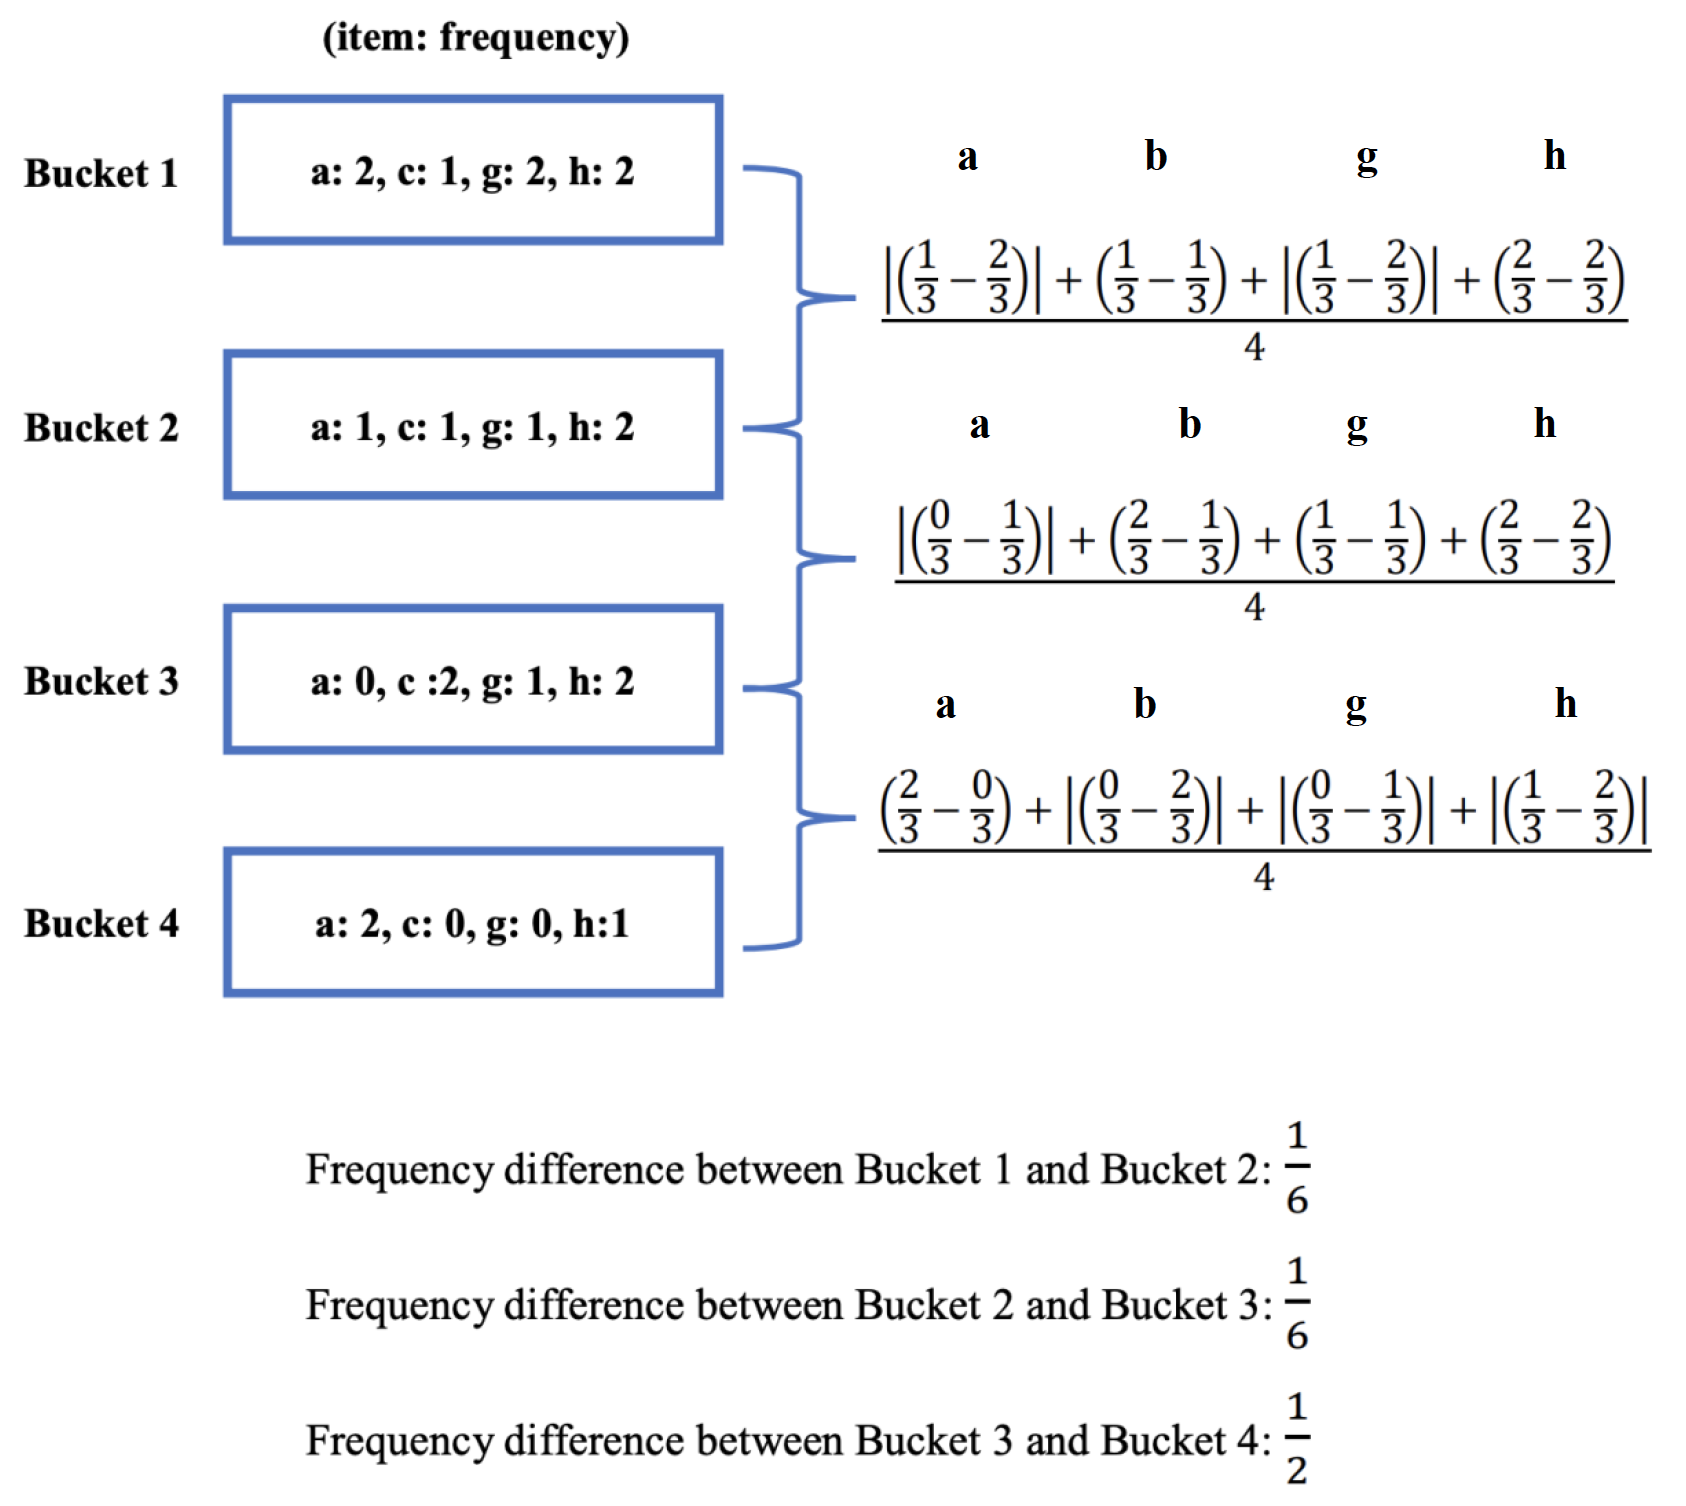
\includegraphics[width=\textwidth]{Methodology/bsc.png}
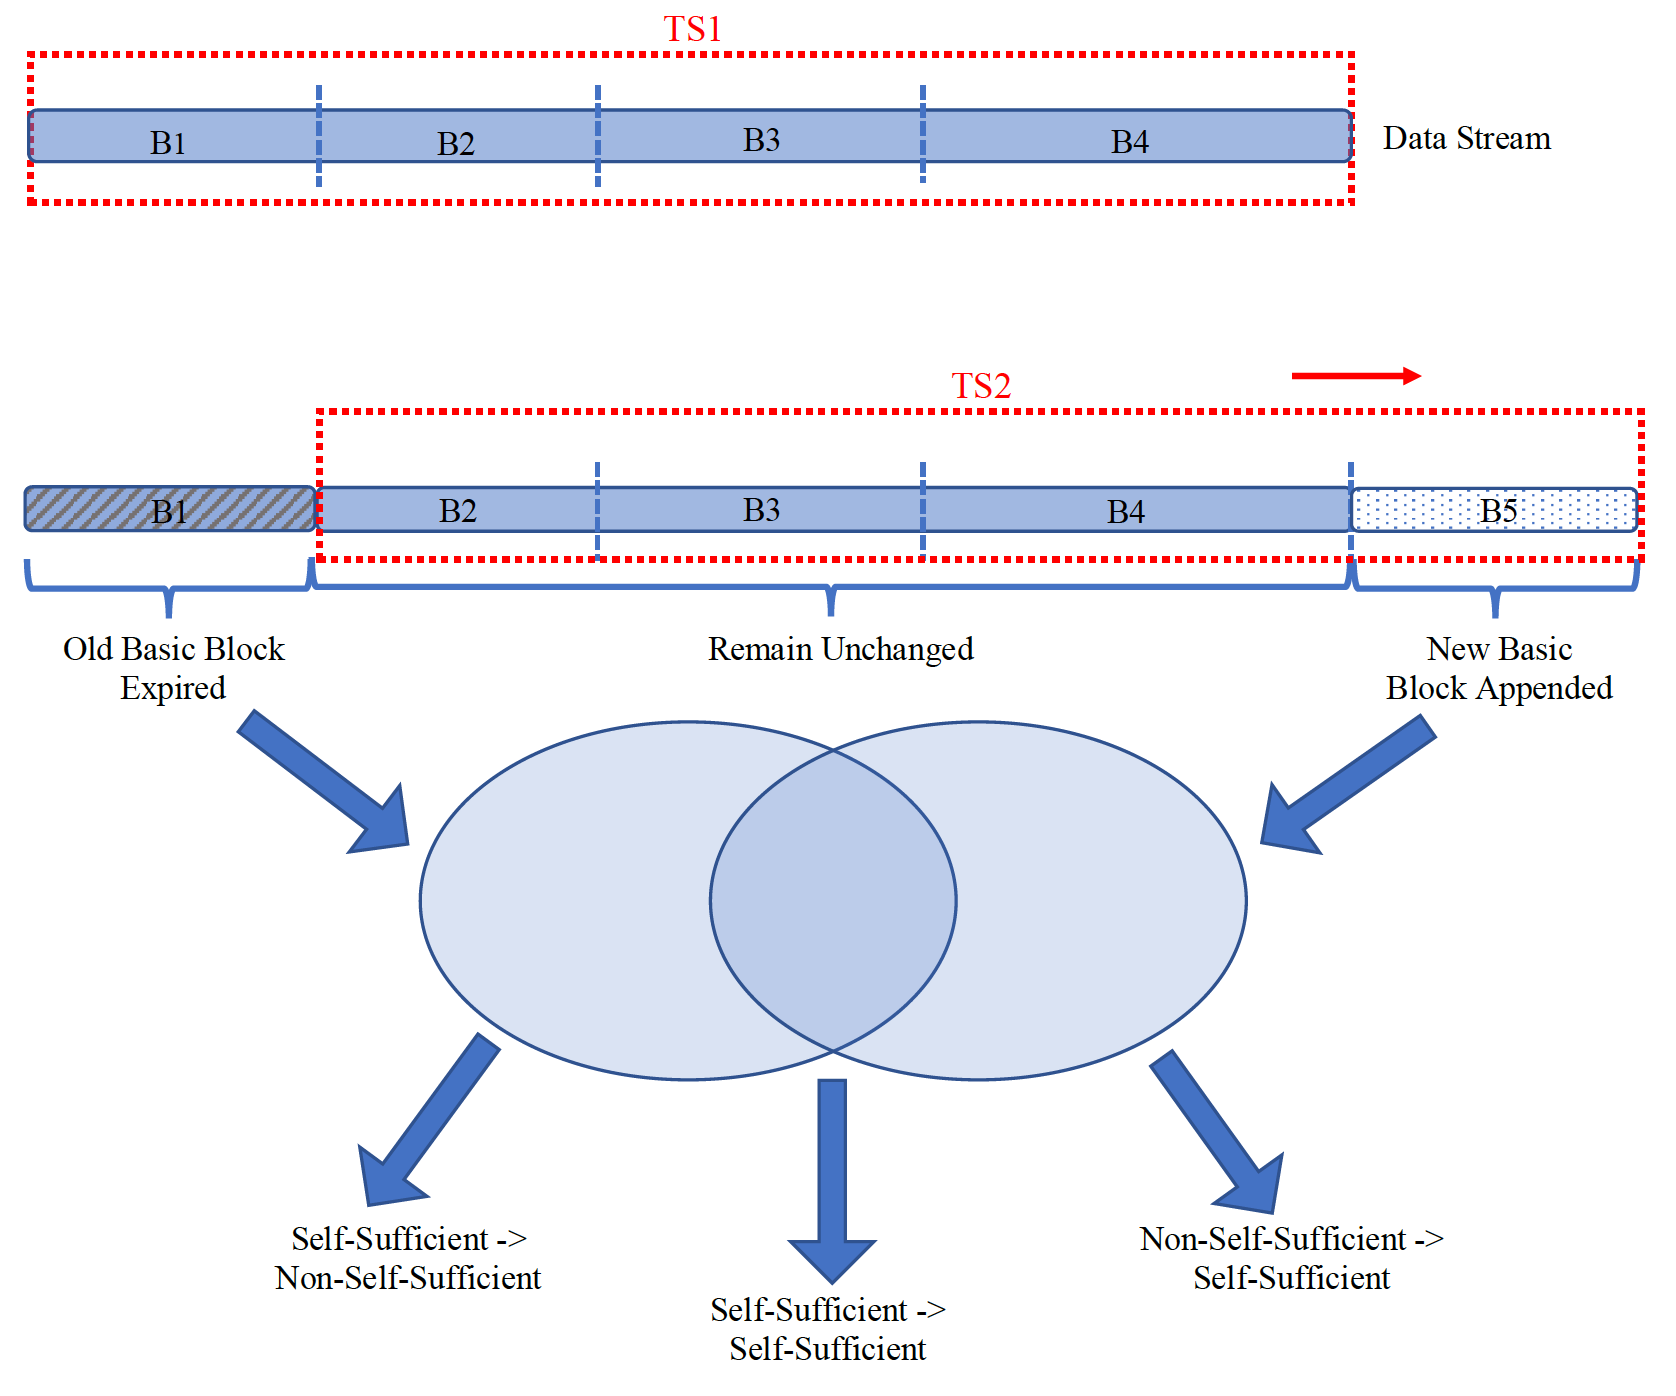
\includegraphics[scale=0.45]{Methodology/TSL.png}
\end{figure}

\subsection{Framework}
Instead of dividing data stream into batches prior to the mining process, Sliding-window Miner (SM) makes some adjustments to help SSIG work in an incremental data stream which achieves the actual real-time mining. 

Consider the two out of three kinds of self-sufficient itemsets mentioned above (the first one has been approved not applicable), we check the appended data stream $B_5$ for self-sufficient itemsets contains new-coming items first. This can be finished by running our SSIG on the appended data stream $B_5$ and store the results.

Next step is to mine itemsets which just turned self-sufficient after the update. These can be those itemsets whose subsets did not have enough associations with the remainder in the expired $B_1$ and remaining $B_2, B_3$. 

In this sliding-window method, we only use the frequency counter of BSC on $TS_1$ to generated a list of frequent items with their frequencies $F$. When $TS_1$ has been fed into SSIG to produce a set of self-sufficient itemsets $S$, the non-expanded items in $F$ will be separated into a new list $F'$. A data stream may be divided into blocks with different numbers of transactions. The buffer continuously consumes transactions and pours them block-by-block into our system. When a new basic block or even a single transaction produced, update $F'$ if it contains any item from $F'$ and feed $F'$ into SSIG to generate new self-sufficient itemsets. This process is illustrated in Fig \ref{fig:smframe}.

\begin{figure}[H]
\caption{How sliding-window miner processes new incoming data}
\label{fig:smframe}
\centering
%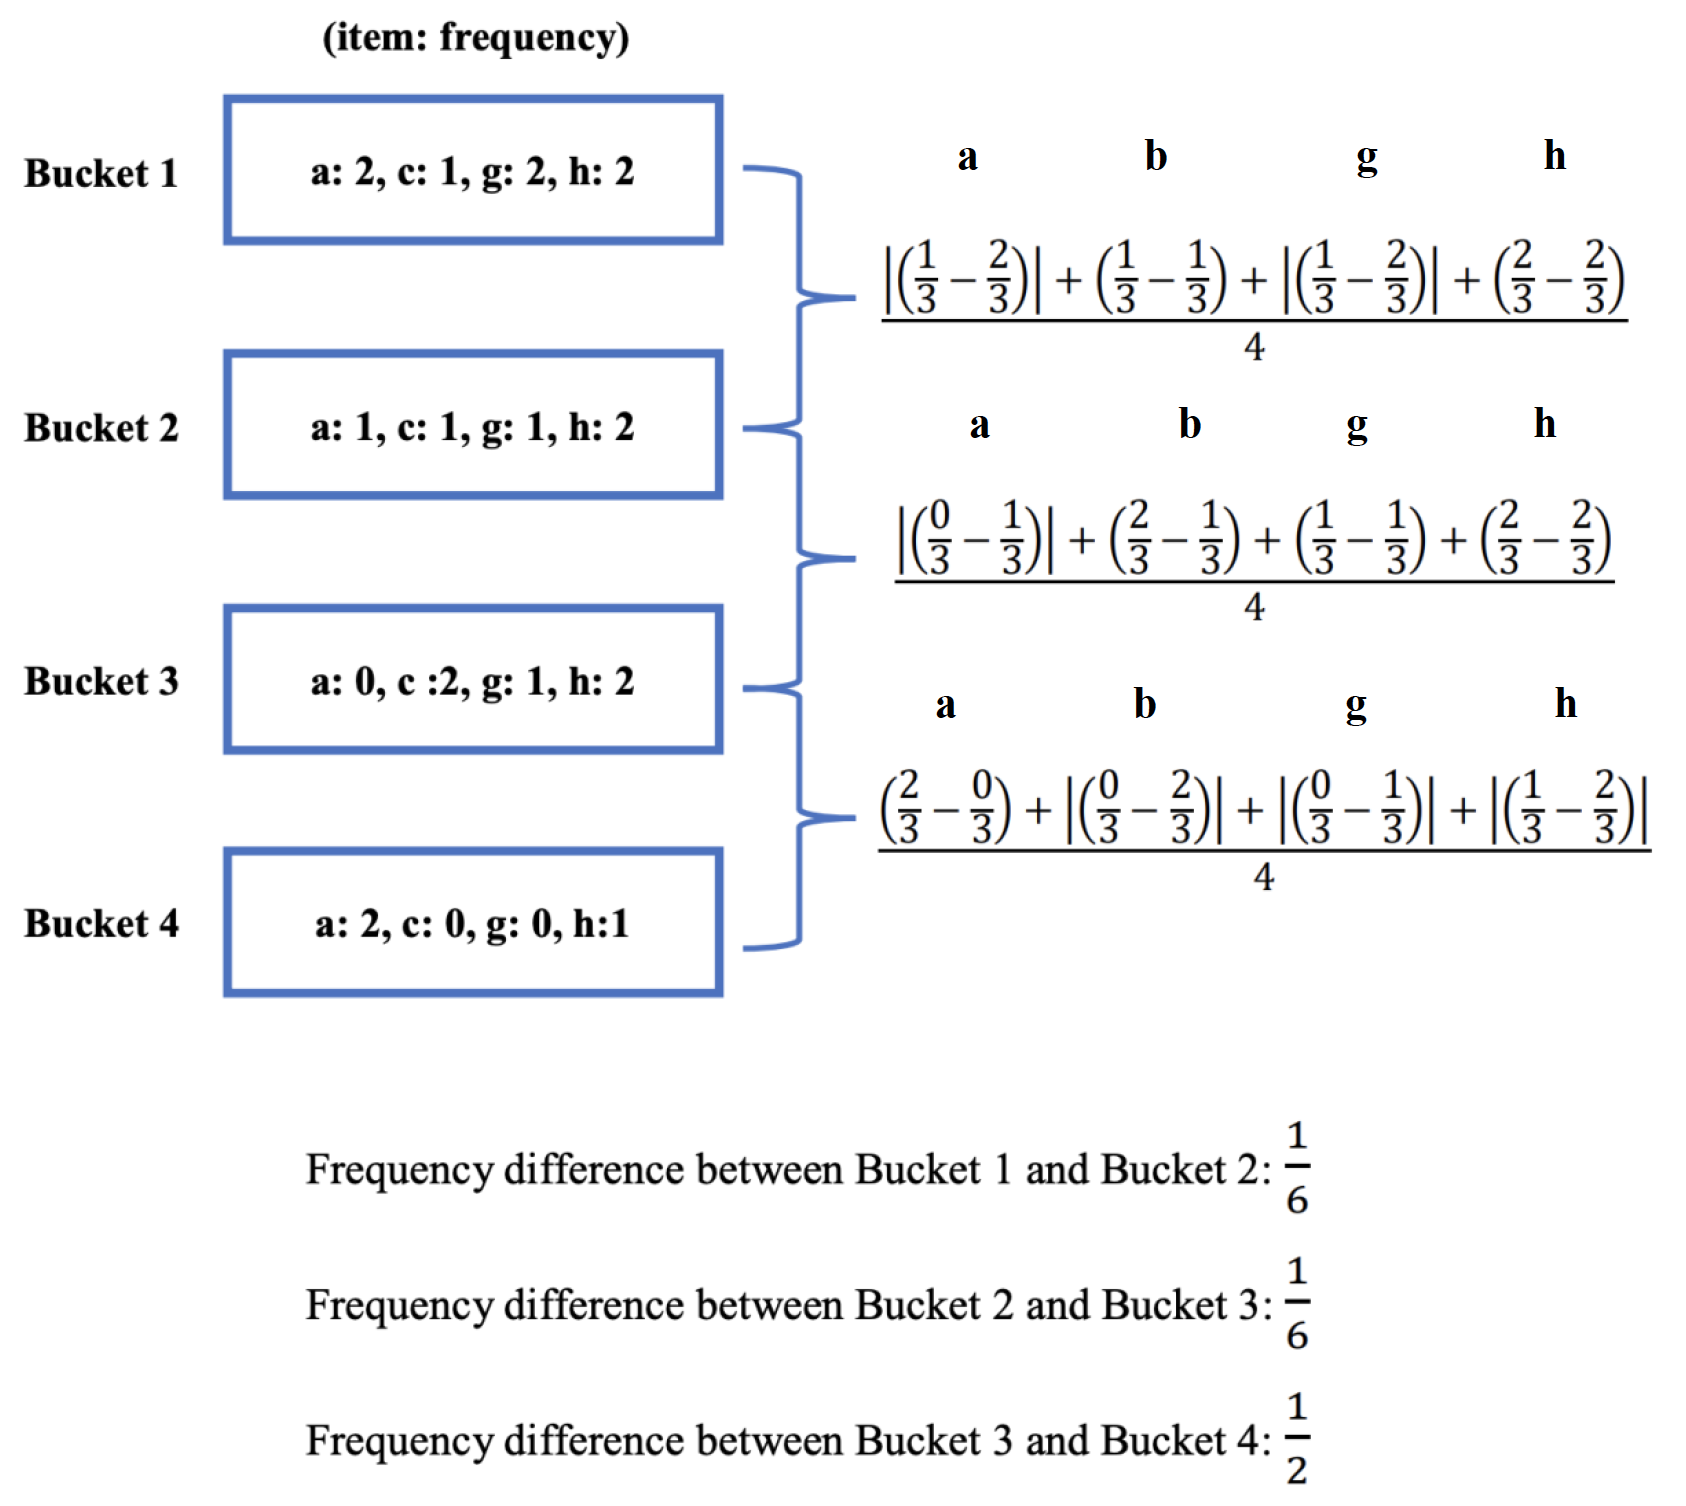
\includegraphics[width=\textwidth]{Methodology/bsc.png}
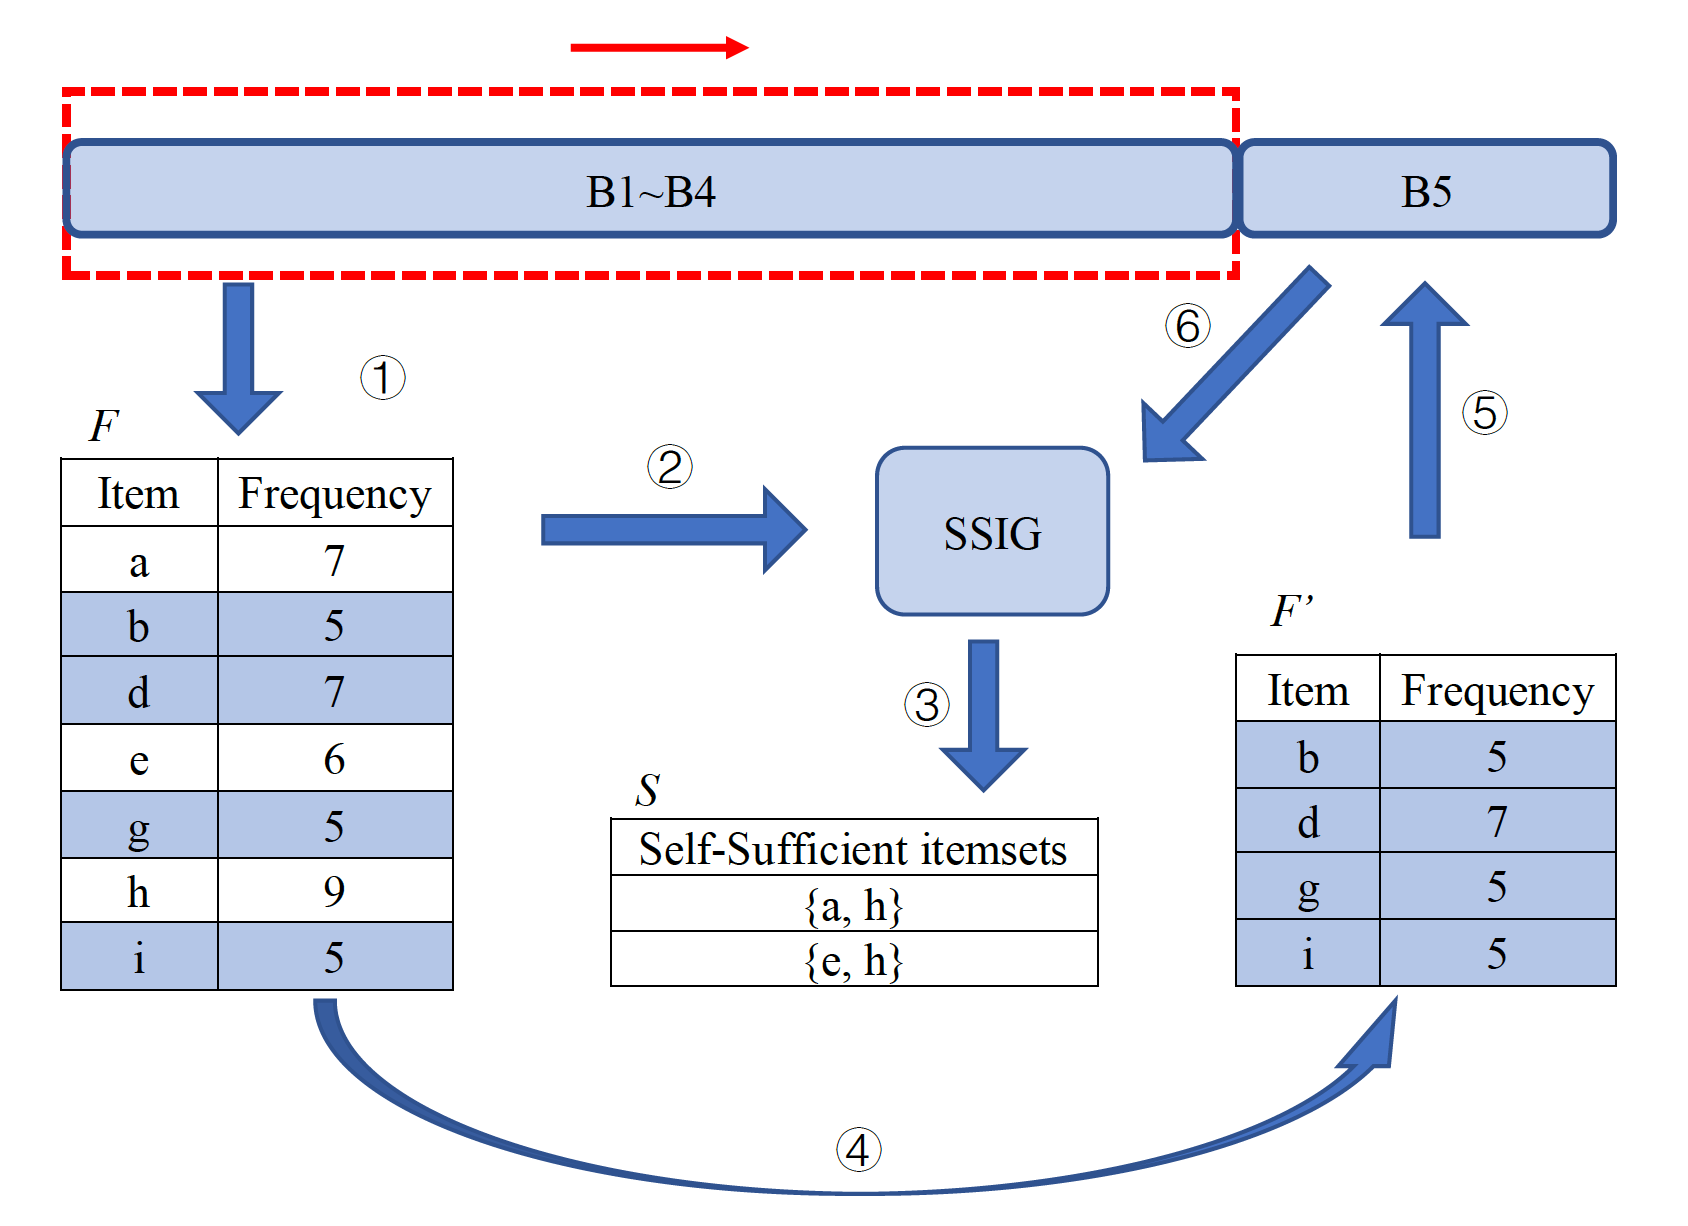
\includegraphics[scale=0.5]{Methodology/frame.png}
\end{figure}

\subsection{Discussion}
Sliding-window Miner has the ability to using a moving window to process data stream incrementally which make up the drawbacks of batch processing we proposed in ASSIM. Because of the limitation of time of this dissertation, we only discuss the Sliding-window Miner technique at the conceptual level. But it is worthy to be developed and experiment its efficiency and compatibility on actual online learning.

\section{Summary}

Interesting association discovery is often a more complicated and computationally expensive task than frequent itemset mining. Besides the traditional ``support-confidence'' framework for association rule mining, the definition of self-sufficient itemset changed the way of determining interestingness of association rules. It is defined as each of a self-sufficient itemset's subset must be associated to its complement. The original efficient self-sufficient miner, also as known as OPUSMiner, achieves an outstanding efficiency, also proved effective and accuracy. While OPUSMiner was developed on a static database, to satisfy the urgent need of data stream adaption, we remedy OPUSMiner by providing a stable batch calculator to produce stable batches and sketch frequent items. To minimise the error brings by underlying distribution changes, also as known as concept drifts in data streams, we added a concept drift adaptor which is able to detect and adapt to underlying drifts. Besides the fact that most mainstream concept drift detector discard data prior to the drift point, which usually miss the regional drift. Our Regional Concept Drift Adaptor provides regional drift detection and adaption for self-sufficient itemset mining. Using batch processing is not actual online learning in fact, we also discussed the sliding-winder miner, which uses a time-sensitive sliding window to mine self-sufficient itemsets from a data stream.

In the next chapter, we will perform several experiments to test the efficiency and effectiveness of our proposed framework.
\chapter{Experiments} \label{chapt:Experiments}

In this section, we describe three groups of experiments conducted to evaluate ASSIM. The first group examines the computational costs of ASSIM, time and memory use. The second group evaluates the accuracy of BSC and RCDA by recording their precision and recall values under difference circumstances. Lastly, we inject different kinds of drifts into the data streams and test the efficiency and accuracy of our drift detector. 

All experiments are conducted on a machine with Intel Core i7-7700 Desktop Processor 4 Cores with up to 4.2 GHz CPU with 32GB RAM.


\section{Descriptions of the Datasets}

\begin{table}[h!]
\caption{Descriptions of the Datasets}
\label{tb:datasets}
\begin{center}
\addtolength{\tabcolsep}{4.0pt}
\begin{tabular}{ll}
    \toprule
    \multirow{1}{*}{Dataset} &
      \multicolumn{1}{l}{Description} \\
      \midrule
    T10I1KD100K & {synthetic dataset with an average transaction length 10}  \\
    T15I1KD1M & {synthetic dataset with an average transaction length 15}  \\
    mushrooms & {prepared based on the UCI mushrooms dataset}  \\
    retail & {retail market basket data from a Belgian retail store}\\
    pumsb & {census data for population and housing}\\
    chess & {prepared based on the UCI chess dataset}\\
    connect & {prepared based on the UCI connect-4 dataset}\\
    accidents & {anonymized traffic accident data}\\
    BMS\_WebView & {click-stream data from a webstore used in KDD-Cup 2000}\\
    chainstore &  {customer transactions from a retail store from NU-Mine Bench}\\
    \bottomrule
\end{tabular}
\end{center}
\end{table}
We employed ten datasets including eight of the largest attribute-value datasets from the UCI machine learning \cite{uci1,uci2} and UCI KDD \cite{uci3} repositories together with the BMS-WebView \cite{bms}, retail \cite{retail} and chainstore from CUCIS\cite{CUCIS} datasets. The other two are synthetic datasets created by IBM data generator. These datasets are described in Table \ref{tb:datasets}. % and Table \ref{tb:datades}.

Each synthetic dataset configuration (\textit{T10I1KD100K} and \textit{T15I1KD1M}) was generated with different seed values and passed into the algorithm 30 times. The other eight real-world datasets were tested a single time each.
% \begin{table}[h!]
% \caption{Dataset Description}
% \label{tb:datades}
% \begin{center}
% \begin{tabular}{lrr}
%     \toprule
%     \multirow{1}{*}{Dataset} &
%       \multicolumn{1}{r}{Record} &
%       \multicolumn{1}{r}{Item} \\
%       \midrule
%     T10I1KD100K & {100,000} & {1,000} \\
%     T15I1KD1M & {1,000,000}& {1,000}\\
%     mushrooms & {8,416} & {119}\\
%     retail & {88,162} & {16,470}\\
%     pumsb & {49,046} & {2,113}\\
%     chess & {3,196} & {75}\\
%     connect & {67,557} & {129}\\
%     accidents & {340,183} & {468}\\
%     BMS\_WebView\_1 & {59,602} & {497}\\
%     chainstore & {1,112,949} & {46,086}\\
%     \bottomrule
% \end{tabular}
% \end{center}
% \end{table}

\section {Runtime and Memory Performance}
We ran our ten datasets on BSC and SSIG separately to record the time and memory used for each component of our technique. In this case, SSIG without batches represents the ground truth which produces the truth result of Self-Sufficient itemsets in each dataset.

Table \ref{tb:time1} %and Table \ref{tb:time2} 
illustrate that BSC works as a stable technique. It has a faster runtime performance as compared from SSIG without batches. In our experiments, the tolerance error rate for the approximation $e=0.05$ and frequency difference threshold $\tau=25\%$.
To further evaluate the efficiency of BSC, we also perform two additional experiments for each dataset. In the additional set of experiments, we feed equally divided batches into SSIG (divided into the same amount of batches as BSC but in fixed interval). This is to show how runtime and memory performance is effected given the same number of datasets. In the second set of experiments, we feed batches into SSIG separately based on the pre-detemined size of the  intervals found using BSC. To do this we noted the location of the batch size found in BSC and then superimposed the same exact batch sizes for SSIG. The significance level $\alpha=0.05$ was used for performing Fisher's Exact Test in SSIG.

This experiments was to evaluate the runtime and memory if we mined at the same time point of BSC.
Table \ref{tb:time1}  shows us that there is no significant difference between the time and memory consumption between SSIG with a fixed interval and with pre-calculated batches based  found using BSC. 

\begin{table}[h!]
\caption{Runtime and Memory Performance}
\label{tb:time1}
\begin{center}
\addtolength{\tabcolsep}{5.0pt}
\begin{tabular}{lrrrr}
    \toprule
    \multirow{2}{*}{Dataset} &
      \multicolumn{2}{c}{BSC} &
      \multicolumn{2}{c}{SSIG without batches} \\
      & {Time (s)} & {Memory (Mb)} & {Time (s)} & {Memory (Mb)} \\
      \midrule
    T10I1KD100K & \textbf{\(1.97\pm 0.92\)} & {\(210.28\pm 0.89\)} & {\(2.85\pm 0.33\)} & {\(148.41\pm 0.33\)} \\
    T15I1KD1M & \textbf{\(35.24\pm 1.36\)} & {\(642.81\pm 2.01\)} & {\(47.42\pm 3.64\)} & {\(572.22\pm 0.97\)} \\
    mushrooms & \textbf{\(0.54\pm 0.04\)} & {\(78.36\pm 0.27\)} & {\(1.09\pm 0.16\)} & {\(55.73\pm 0.21\)} \\
    retail & \textbf{\(1.64 \pm 0.29\)} & {\(192.45\pm 0.84\)}& {\(2.44\pm 1.02\)} & {\(136.85\pm 0.76\)}\\
    pumsb & \textbf{\(0.92\pm 0.05\)} & {\(101.34\pm0.76\)}& {\(1.49\pm0.11\)} & {\(74.32\pm 0.19\)}\\
    chess & \textbf{\(0.19\pm0.02\)} & {\(25.92\pm0.37\)}& {\(0.31\pm0.10\)} & {\(10.78\pm0.14\)}\\
    connect & \textbf{\(1.85\pm 0.06\)} & {\(168.32\pm1.92\)}& {\(2.11\pm 0.21\)} & {\(103.27\pm0.35\)}\\
    accidents & \textbf{\(8.24\pm0.79\)} & {\(385.56\pm2.34\)}& {\(2.87\pm0.67\)} & {\(339.14\pm0.68\)}\\
    BMS\_WebView & \textbf{\(1.11\pm0.12\)} & {\(119.38\pm0.78\)}& {\(1.46\pm0.40\)} & {\(91.25\pm0.07\)}\\
    chainstore & \textbf{\(38.21\pm1.28\)} & {\(783.15\pm2.35\)}& {\(51.97\pm2.07\)} & {\(711.92\pm1.06\)}\\
    \bottomrule
\end{tabular}
% \end{center}
% \end{table}

\noalign{\smallskip}

% \begin{table}[h!]
% \caption{Time and Memory Use}
% \label{tb:time2}
% \begin{center}
\begin{tabular}{lrrrr}
    \toprule
    \multirow{2}{*}{Dataset} &
      \multicolumn{2}{c}{SSIG with fixed intervals} &
      \multicolumn{2}{c}{SSIG with batches} \\
      & {Time (s)} & {Memory (Mb)} & {Time (s)} & {Memory (Mb)} \\
      \midrule
    T10I1KD100K & {\(3.04\pm 0.69\)} & {\(149.12\pm 0.30\)} & {\(3.05\pm 0.23\)} & {\(149.10\pm 0.27\)} \\
    T15I1KD1M & {\(49.10\pm 2.41\)} & {\(574.11\pm 0.85\)} & {\(49.17\pm 1.94\)} & {\(574.12\pm 0.88\)} \\
    mushrooms & {\(1.15\pm 0.11\)} & {\(56.09\pm 0.33\)} & {\(1.17\pm 0.23\)} & {\(56.12\pm 0.19\)} \\
    retail & {\(2.69 \pm 0.27\)} & {\(138.02\pm 0.81\)}& {\(2.82\pm 0.04\)} & {\(137.98\pm 0.84\)}\\
    pumsb & {\(1.52\pm 0.11\)} & {\(75.65\pm0.22\)}& {\(1.52\pm0.12\)} & {\(75.61\pm 0.27\)}\\
    chess & {\(0.39\pm0.02\)} & {\(10.98\pm0.07\)}& {\(0.39\pm0.04\)} & {\(11.02\pm0.08\)}\\
    connect & {\(2.30\pm 0.10\)} & {\(104.25\pm0.29\)}& {\(2.28\pm0.09\)} & {\(104.23\pm0.33\)}\\
    accidents & {\(3.02\pm0.32\)} & {\(321.01\pm0.72\)}& {\(2.99\pm0.17\)} & {\(320.88\pm0.77\)}\\
    BMS\_WebView & {\(1.57\pm0.07\)} & {\(92.07\pm0.15\)}& {\(1.57\pm0.12\)} & {\(92.05\pm0.17\)}\\
    chainstore & {\(56.39\pm0.27\)} & {\(714.24\pm0.84\)}& {\(56.41\pm0.19\)} & {\(714.25\pm0.86\)}\\
    \bottomrule
\end{tabular}
\end{center}
\end{table}




\section{Experiments to Evaluate Precision and Recall}
As a result of using Lossy Counting \cite{lossy} in BSC, all the frequent items produced by BSC are true positives. Thus producing 100\% precision. Lossy Counting in BSC only provides an approximation to the frequency of an items a batch. Some of the frequent items, which should have been included for expansion to Self-Sufficient itemsets may be missed. This would lead to  recall being less than 100\%. We use the SSIG without batches as the ground truth of the set of self-sufficient itemsets found. 

\begin{table}[h!]
\caption{Precision and Recall}
\label{tb:pr1}
\begin{center}
\resizebox{\textwidth}{!}{
\begin{tabular}{lrrrrrr}
    \toprule
    \multirow{2}{*}{Dataset} &
    \multicolumn{2}{c}{BSC} &
      \multicolumn{2}{c}{SSIG with fixed intervals} &
      \multicolumn{2}{c}{SSIG with batches} \\
  & {Precision (\%)} & {Recall (\%)}
      & {Precision (\%)} & {Recall (\%)}& {Precision (\%)} & {Recall (\%)} \\
      \midrule
    T10I1KD100K & {\(100\%\pm 0\%\)} & {\(97\%\pm 2\%\)}& {\(96\%\pm 1\%\)} & {\(98\%\pm 2\%\)}& {\(97\%\pm 2\%\)} & {\(98\%\pm 1\%\)} \\
    T15I1KD1M & {\(100\%\pm 0\%\)} & {\(98\%\pm 1\%\)} &{\(93\%\pm 3\%\)} & {\(95\%\pm 4\%\)} & {\(96\%\pm 2\%\)} & {\(99\%\pm 1\%\)} \\
    
    \noalign{\smallskip}\hline\noalign{\smallskip}
    
    mushrooms & {\(100\%\)} & {\(97\%\)} &{\(97\%\)} & {\(99\%\)} & {\(97\%\)} & {\(97\%\)}\\
    retail & {\(100\%\)} & {\(98\%\)} &{\(95\%\)} & {\(96\%\)} & {\(97\%\)} & {\(97\%\)}\\
    pumsb & {\(100\%\)} & {\(98\%\)} &{\(96\%\)} & {\(94\%\)} & {\(97\%\)} & {\(94\%\)}\\
    chess & {\(100\%\)} & {\(100\%\)} &{\(100\%\)} & {\(98\%\)} & {\(100\%\)} & {\(99\%\)}\\
    connect & {\(100\%\)} & {\(98\%\)} & {\(95\%\)} & {\(97\%\)} & {\(95\%\)} & {\(97\%\)}\\
    accidents &{\(100\%\)} & {\(96\%\)} &  {\(93\%\)} & {\(94\%\)} & {\(98\%\)} & {\(98\%\)}\\
    BMS\_WebView & {\(100\%\)} & {\(99\%\)} &{\(96\%\)} & {\(95\%\)} & {\(99\%\)} & {\(97\%\)}\\
    chainstore & {\(100\%\)} & {\(95\%\)} &{\(95\%\)} & {\(97\%\)} & {\(96\%\)} & {\(99\%\)}\\
    \bottomrule
\end{tabular}}
\end{center}
\end{table}


With the batch calculation from BSC, the correctly detected batches of data stream achieved better precision and recall values for Self-Sufficient itemset mining as compared to SSIG with fixed intervals or SSIG with batches.

\section {Experiments to Evaluate the Regional Drift Detection}
In the drift detection part, we perform two different tests: abrupt and gradual drift detection on \textit{T10I1KD100K} dataset. The delta value $\delta=0.002$ was set for ADWIN drift detector. For abrupt drifts, we inject different numbers of abrupt drifts, specifically 5, 10 and 20 into \textit{T10I1KD100K}. Several indications were recorded: time and memory costs, true and false positives, and delay. Based on the results the increase of  drift points, this leads to worse false positives.

To evaluate gradual drift detection, we used the same dataset \textit{T10I1KD100K} but changed data in different rates noted as the slopes, specifically 250, 500 and 1,000. Same indications were used for this test, and it showed that higher slopes produce worse false positives and longer delay.

\begin{table}[h!]
\caption{Abrupt Drift Detection}
\label{tb:abrupt}
\begin{center}
\resizebox{\textwidth}{!}{
\begin{tabular}{lrrrrr}
    \toprule
    \multirow{1}{*}{\#Drifts} &
      \multicolumn{1}{c}{Time (s)} &
      \multicolumn{1}{c}{Memory (Mb)} &
      \multicolumn{1}{c}{TP Rate (\%)} &
      \multicolumn{1}{c}{FP} &
      \multicolumn{1}{c}{Delay}\\
      \midrule
    5 & {\(6.42\pm 0.11\)} & {\(23.1\pm 0.07\)} & {\(1.0\pm 0.00\)} & {\(77.81\pm 0.07\)} & {\(184.65\pm 67.84\)}\\
    10 & {\(6.54\pm 0.08\)} & {\(23.2\pm 0.09\)} & {\(1.0\pm 0.00\)} & {\(385.42\pm 39.61\)} & {\(157.82\pm 39.61\)}\\
    20 & {\(6.59\pm 0.10\)} & {\(23.1\pm 0.08\)} & {\(1.0\pm 0.00\)} & {\(793.11\pm 55.28\)} & {\(93.11\pm 35.28\)}\\
    \bottomrule
 \end{tabular}
 }
\end{center}
\end{table}


\begin{table}[h!]
\caption{Gradual Drift Detection}
\label{tb:gradual}
\begin{center}
\resizebox{\textwidth}{!}{
\begin{tabular}{lrrrrr}
    \toprule
    \multirow{1}{*}{Slope} &
      \multicolumn{1}{c}{Time (s)} &
      \multicolumn{1}{c}{Memory (Mb)} &
      \multicolumn{1}{c}{TP Rate (\%)} &
      \multicolumn{1}{c}{FP} &
      \multicolumn{1}{c}{Delay}\\
      \midrule
    250 & {\(6.52\pm 0.14\)} & {\(23.1\pm 0.03\)} & {\(1.0\pm 0.00\)} & {\(174.29\pm 53.11\)} & {\(98.35\pm 78.25\)}\\
    500 & {\(6.82\pm 0.18\)} & {\(23.2\pm 0.07\)} & {\(1.0\pm 0.00\)} & {\(482.36\pm 42.83\)} & {\(164.70\pm 69.83\)}\\
    1000 & {\(7.01\pm 0.22\)} & {\(23.1\pm 0.03\)} & {\(1.0\pm 0.00\)} & {\(853.16\pm 107.28\)} & {\(218.65\pm 109.62\)}\\
    \bottomrule
 \end{tabular}
 }
\end{center}
\end{table}

\section{Case Study: USCensus}

This dataset is transformed from the US Census 1990 dataset, obtained from UCI Machine Learning Repository~\cite{uci1,uci2}, where 1,000,000 instances were transformed to transactions, and where there are 396 distinct items. Figure \ref{fig:frequs} shows the normalised item frequency distribution of the USCensus dataset. When we compared the distribution of the USCensus dataset, to other commonly used data mining datasets, we observed that the USCensus dataset is much more sparse in nature compared to the other real-world datasets we used to perform experiments, but more dense than datasets like Kosarak. Because of its sparsity, it is interesting to see how this could potentially affect the Self-Sufficient itemset mining process. 

\begin{figure}[H]
    \centering
    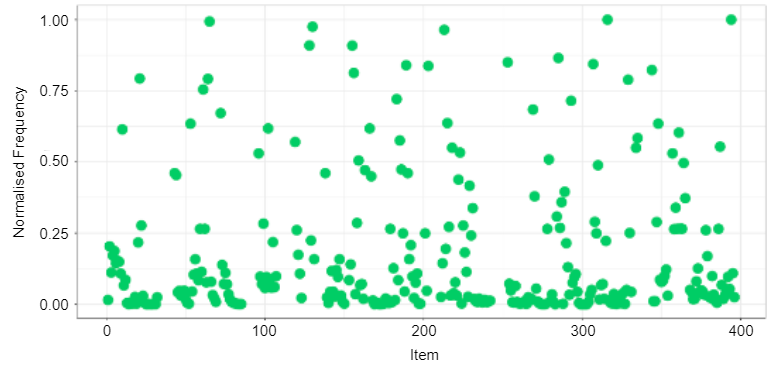
\includegraphics[width=0.9\textwidth]{Experiments/Frequencynor.png}
    \caption{Normalised item frequency distribution}
    \label{fig:frequs}
\end{figure}

\subsection{Runtime and Memory Performance}
We ran USCensus on BSC and SSIG separately to record the time and memory used for each component of our technique. Table \ref{tb:time2} illustrates that for a very sparse dataset like USCensus, BSC with SSIG may need a longer time to divide batches but the difference before and after adding BSC is not very significant.

\begin{table}[h!]
\caption{Runtime and Memory Performance for USCensus}
\label{tb:time2}
\begin{center}
\addtolength{\tabcolsep}{5.0pt}
\begin{tabular}{lrrrr}
    \toprule
    \multirow{2}{*}{Dataset} &
      \multicolumn{2}{c}{BSC} &
      \multicolumn{2}{c}{SSIG without batches} \\
      & {Time (s)} & {Memory (Mb)} & {Time (s)} & {Memory (Mb)} \\
      \midrule
    USCensus & \textbf{\(32.81\pm 0.94\)} & {\(654.27\pm 3.11\)} & {\(32.25\pm 1.63\)} & {\(584.74\pm 1.16\)} \\
    \bottomrule
\end{tabular}


\noalign{\smallskip}

\begin{tabular}{lrrrr}
    \toprule
    \multirow{2}{*}{Dataset} &
      \multicolumn{2}{c}{SSIG with fixed intervals} &
      \multicolumn{2}{c}{SSIG with batches} \\
      & {Time (s)} & {Memory (Mb)} & {Time (s)} & {Memory (Mb)} \\
      \midrule
    USCensus & {\(33.71\pm 1.22\)} & {\(661.32\pm 0.51\)} & {\(33.25\pm 0.43\)} & {\(659.10\pm 0.44\)} \\
    \bottomrule
\end{tabular}
\end{center}
\end{table}

\subsection{Experiments to Evaluate Precision and Recall}

Same as we discussed before, the results came out from BSC are guaranteed to be frequent which guarantees a 100\% precision. Because most of the items in USCensus are infrequent with a less than 0.1 frequency, the recall of BSC performs well - very frequent items are easy to be found. 

BSC provides specific calculations on the distribution change points for frequent items which directly help SSIG with the Self-Sufficient itemset mining process. According to \ref{tb:prrc}, these properly divided batches of USCensus achieved a much better precision and recall values for Self-Sufficient itemset mining comparing to the ground truth (SSIG with fixed intervals).

\begin{table}[h!]
\caption{Precision and Recall for USCensus}
\label{tb:prrc}
\begin{center}
\resizebox{\textwidth}{!}{
\begin{tabular}{lrrrrrr}
    \toprule
    \multirow{2}{*}{Dataset} &
    \multicolumn{2}{c}{BSC} &
      \multicolumn{2}{c}{SSIG with fixed intervals} &
      \multicolumn{2}{c}{SSIG with batches} \\
  & {Precision (\%)} & {Recall (\%)}
      & {Precision (\%)} & {Recall (\%)}& {Precision (\%)} & {Recall (\%)} \\
      \midrule
    USCensus & {\(100\%\)} & {\(97\%\)} &{\(92\%\)} & {\(95\%\)} & {\(96\%\)} & {\(98\%\)}\\
    \bottomrule
\end{tabular}}
\end{center}
\end{table}


\section{Conclusion}

In this section I conducted several experiments to test the performance of ASSIM by comparing the runtime and memory use, precision and recall rates and drift detection accuracy. From the runtime and memory experiments, I concluded that there is no significant difference between the time and memory consumption between with or without using Batch Size Calculator, which shows ASSIM does not requires extra computation cost. I then evaluated the precision and recall rates, data stream with correctly divided batches achieved better precision and recall values for Self-Sufficient itemset mining than using no ASSIM. Finally, I tested our regional drift detector which also achieved promising results. My case study on US Census data also showed similar results as before, proved that ASSIM works as a stable and workable framework.


\chapter{Conclusion} \label{chapt:Conclusion}

In this dissertation, we first comprehensively reviewed the pure ``support-confidence" framework for pattern mining and proposed a novel solution - self-sufficient itemsets. Then, we highlighted the deficiencies of the current methods. Against the shortage of current methods, we proposed Adaptive Self-Sufficient Itemset Miner (ASSIM) which makes self-sufficient itemset miner work in an online mode along with a drift detector to reduce the error brought by the non-stationary distributions. ASSIM includes a Batch Size Calculator to calculate the size of the batches, Self-Sufficient Itemset Generator to mine Self-Sufficient itemsets and Regional Concept Drift Adaptor to detect regional concept drifts.

Experiments demonstrated that the Batch Size Calculator provides more accurate results without substantially increasing time or memory consumption. This proves that our technique ASSIM could achieve a better result as compared to using the Self-Sufficient itemset miners in a static way.

In this final chapter we summarise our fndings and results presented in the dissertation, and discuss future directions for our research.

\section{Achievements} \label{Conclusion:Achievements}

The following list highlights the major achievements of this project:
\begin{itemize}
	\item We proposed a new framework ASSIM that is able to mine self-sufficient itemset from unlabelled item-based transactional data streams.
		
	\item We presented a new approach that enables the detection of self-sufficient itemset drifts from unlabelled item-based transactional data streams.
	
	\item We proposed a new regional drift detector that detects and adapts regional drifts in self-sufficient itemset mining to the underlying regional concept drifts.
	
	\item Through our evaluation, we showed that our design is feasible and improved the performance of the overall self-sufficient itemset mining and concept drift detection process by significantly improving precision and recall rates.
	
\end{itemize}

\section{Limitations} \label{Conclusion:Limitations}

This dissertation has presented algorithms and approaches that contribute to solving problems in change mining for the data stream environment. Despite the contributions, there are some limitations to the proposed algorithms and approaches.

The first limitation is related to the concept drift detection for self-sufficient itemset mining. The current methodology works to detect drifts on a single mined self-sufficient itemset for each round, which can cause extra computational cost and complicate the process. It might be possible to perform this task on a parallel mode which can run multiple drift detectors on the same time.

The second limitation is related to the actual online learning. As we discussed before in Chapter \ref{chapt:ASSIM}, it is possible to adopt a sliding-window model to actual achieve both the self-sufficient itemset and drift adaption process on a real-time updating data stream.

\section{Future Directions} \label{Conclusion:FutureDirections}

There are several future directions for the work this thesis presents. We will first discuss the future work for each of the individual topics in the chapters followed by broader general future directions we wish to pursue.

\paragraph{Association Rule Mining}

We discussed in detail how to find self-sufficient itemsets from unsupervised data streams in Chapter \ref{chapt:ASSIM}. In the future we intend to investigate dynamically adapting the $k$ value of our proposed technique based on the feature of data stream. For example, it is possible that a data stream contains more than 100 self-sufficient itemsets but the actual association rules needed are only 50. In this case, it is important to apply a filter on the preparation stage of data stream processing to give $k$ a tighter bound.

\paragraph{Regional Drift Mining}

We proposed a Regional Concept Drift Adaptor (RCDA) to facilitate the discovery of item association changes of self-sufficient itemsets in Chapter \ref{chapt:ASSIM}. Our future work in this part includes developing a more accurate method for regional drift adaptor which can retrieve location information related to drifted regions. This information can then be used to analyse in a wider picture to build a more accurate adaptive self-sufficient itemset miner that can better handle real-world data streams. We also want to adapt RCDA on a parallel mode to apply on multiple self-sufficient itemset on a single round.



\backmatter
\bibliographystyle{plain}
\addcontentsline{toc}{chapter}{Bibliography}
\bibliography{bibliography}


\end{document}